% $HeadURL$

\chapter{Process Description Glyphs}
\label{chp:glyphs}

%[Note on the color code: \textcolor{blue}{The glyphs that have been thoroughly discussed, and are considered frozen, are represented in blue}. \textcolor{green}{The glyphs that have been thorougly discussed, but are still posing problems are represented in green}. \textcolor{red}{The glyphs that have been proposed but for which in-depth discussion is yet to come are represented in red}.]


\section{Overview}

To set the stage for what follows in this chapter, we give first a brief overview of some of the concepts in the \PDl with the help of an example shown in \fig{eg1}.

\begin{figure}[H]
  \centering
  \includegraphics[scale=0.7]{images/build/MAPK_only_example.pdf}
  \caption{This example of a \PD map uses two kinds of entity pool nodes: one
    for pools of different macromolecules (\sect{macromolecule}) and
    another for pools of simple chemicals (\sect{simpleChemical}).  Most
    \glyph{macromolecule} nodes in this map are adorned with \glyph{state
    variables} (\sect{stateVariable}) representing phosphorylation states.
    This map uses one type of \glyph{process node}, the \glyph{process} node
    (\sect{process}), and three kinds of connecting arc, \glyph{consumption} (\sect{consumption}), \glyph{production} (\sect{production}) and \glyph{catalysis}
    (\sect{catalysis}).  Finally, some entity pool nodes have dark bands
    along their bottoms; these are \glyph{clone markers} (\sect{cloneMarker}) indicating that the same
    pool nodes appear multiple times in the map.}
  \label{fig:eg1}
\end{figure}

The map in \fig{eg1} is a simple map for part of a mitogen-activated protein kinase (MAPK) cascade.  The larger nodes in the figure (some of which are in the shape of rounded rectangles and others in the shape of circles) represent biological materials---things like macromolecules and simple chemicals.  The biological materials are altered via processes, which are indicated in \PDl by lines with arrows and other decorations.  In this particular map, all of the processes happen to be the same: processes catalysed by biochemical entities.  The directions of the arrows indicate the direction of the processes; for example, unphosphorylated RAF kinase processes to phosphorylated RAF kinase via a process catalysed by RAS. Although ATP and ADP are shown as incidental to the phosphorylations on this particular graph, they are involved in the same process as the proteins getting phosphorylated. The small circles on the nodes for RAF and other entity pools represent state variables (in this case, phosphorylation sites). 

The essence of the \PDs is the \emph{change}: it shows how different entities in the system process from one form to another.  The entities themselves can be many different things.  In the example of \fig{eg1}, they are pools of either macromolecules or simple chemicals, but as will become clear later in this chapter, they can be other conceptual and material constructs as well.  Note also that we speak of \emph{entity pools} rather than individuals; this is because, in biochemical network models, one does not focus on single molecules, but rather collections of molecules of the same kind.  The molecules in a given pool are considered indistinguishable from each other.  The way in which one type of entity is transformed into another is conveyed by a \emph{process node} and links between entity pool nodes, and process nodes indicate influence by the entities on the processes.  In the case of \fig{eg1}, those links describe consumption \sect{consumption}, production \sect{production} and catalysis \sect{catalysis}, but others are possible.  Finally, nodes in \PDs are usually not repeated; if they do need to be repeated, they are marked with \emph{clone markers}---specific modifications to the appearance of the node (\sect{cloneMarker}). The details of this and other aspects of \PD notation are explained in the rest of this chapter.

\tab{component-summary} summarizes the different SBGN abstractions described in this chapter.

\newcolumntype{P}[1]{>{\raggedright\hspace{0pt}\arraybackslash}p{#1}}

\begin{table}[bh]
  \centering
  \small
  \begin{tabular}{@{}llP{2.4in}P{1.6in}@{}}
    \toprule
    \textbf{Component} & \textbf{Abbrev.} & \textbf{Role} & \textbf{Examples}\\
    \midrule
    Entity pool node
    & EPN
    & A population of entities that cannot be distinguished from each other
    & Specific macromolecules or other chemical species \\[0.5em]

    Container node	
    % 
    & CN
    & An encapsulation of one or more other SBGN constructs
    & Compartments \\[1.6em]

    Process node
    & PN
    & A process that transforms one or more EPNs into one or more other EPNs
    & Process, association, dissociation \\[0.5em]

    Arc
    & ---
    & Links between EPNs, CNs or Logical Operators to PNs or Logical operators
    & Production, catalysis, inhibition \\[0.5em]

    Logical operators
    & LO
    & Combines one or several inputs into one output
    & Boolean \emph{and}, \emph{or}, \emph{not} \\
    \bottomrule
  \end{tabular}
  \caption{Summary of \PD components and their roles.}
  \label{tab:component-summary}
\end{table}


\section{Controlled vocabularies used in \SBGNPDLone}\label{sec:CVs}

%%%%%%%%%%%%%%%%%%%%%%%%%%%%%%%%%%%%%%%%%%%%%%%%%%%%%%%%%%%%%%%%%%%%%%
%%%%                   Controlled vocabularies
%%%%%%%%%%%%%%%%%%%%%%%%%%%%%%%%%%%%%%%%%%%%%%%%%%%%%%%%%%%%%%%%%%%%%%
%\color{blue}

Some glyphs in SBGN \PDs can contain particular kinds of textual annotations conveying information relevant to the purpose of the glyph.  These annotations are \glyph{units of information} (\sect{unitInfo}) or \glyph{state variables}  (\sect{stateVariable}).  For example, multimers can have a unit of information conveying the number of monomers composing the multimer. 

Other cases are described throughout the rest of this chapter.

The text that appears as the unit of information decorating an Entity Pool Node (EPN) must in most cases be prefixed with a controlled vocabulary term indicating the type of information being expressed.  The prefixes are mandatory except in the case of macromolecule covalent modifications (\sect{covalent-mod-cv}).  
Without the use of controlled vocabulary prefixes, it would be necessary to have different glyphs to indicate different classes of information; this would lead to an explosion in the number of symbols needed.

In the rest of this section, we describe the controlled vocabularies (CVs) used in \SBGNPDLone.  
They cover the following categories of information: an EPN's material type, an EPN's conceptual type, covalent modifications on macromolecules, the physical characteristics of compartments, and cardinality (\eg of multimers).  
In each case, some CV terms are predefined by SBGN, but unless otherwise noted, \emph{they are not the only terms permitted}.  
Users may use other CV values not listed here.
In such cases, they should explain the term's meanings in a figure legend or other text accompanying the map.
% 
Users of CV values not listed here should \emph{strongly} attempt different prefixes from those listed in this document. 


\subsection{Entity pool node material types}
\label{sec:material-types-cv}

The material type of an EPN indicates its chemical structure and physical composition.  A list of common material types is shown in \tab{material-types-cv}, but others are possible.  The values are to be taken from the \sbo (\sbourl), specifically from the branch having identifier \sboid{SBO:0000240} (the \emph{material entity} under \emph{entity}).

\begin{table}[h]
  \centering
  \begin{tabular}{l>{\ttfamily}l>{\ttfamily}l}
    \toprule
    \textbf{Name}              & \textbf{\rmfamily Label} & \textbf{\rmfamily SBO term} \\
    \midrule
    Non-macromolecular ion     & mt:ion  & SBO:0000327\\
    Non-macromolecular radical & mt:rad  & SBO:0000328\\
    Ribonucleic acid           & mt:rna  & SBO:0000250\\
    Deoxyribonucleic acid       & mt:dna  & SBO:0000251\\
    Protein                    & mt:prot & SBO:0000297\\
    Polysaccharide             & mt:psac & SBO:0000249\\
    \bottomrule
  \end{tabular}
  \caption{A sample of values from the \emph{material types} controlled
    vocabulary (\sect{material-types-cv}).}
  \label{tab:material-types-cv}
\end{table}

The material types are in contrast to the \emph{conceptual types} (see below).  The distinction is that material types are about physical composition, while conceptual types are about roles.  For example, a strand of RNA is a material type, but its use as messenger RNA is a role.


\subsection{Entity pool node conceptual types}
\label{sec:conceptual-types-cv}

An EPN's \emph{conceptual type} indicates its function within the context of a given \PD.  A list of common conceptual types is shown in \tab{conceptual-types-cv}, but others are possible.  The values are to be taken from the \sbo (\sbourl), specifically from the branch having identifier \sboid{SBO:0000241} (the \emph{conceptual entity} under \emph{entity}).  

\begin{table}[h]
  \centering
  \begin{tabular}{l>{\ttfamily}l>{\ttfamily}l}
    \toprule
    \textbf{Name}              & \textbf{\rmfamily Label} & \textbf{\rmfamily SBO term} \\
    \midrule
    Gene                      & ct:gene   & SBO:0000243\\
    Transcription start site  & ct:tss    & SBO:0000329\\
    Gene coding region        & ct:coding & SBO:0000335\\
    Gene regulatory region    & ct:grr    & SBO:0000369\\
    Messenger RNA             & ct:mRNA   & SBO:0000278\\
    \bottomrule
  \end{tabular}
  \caption{A sample of values from the \emph{conceptual types} vocabulary
    (\sect{conceptual-types-cv}).}
  \label{tab:conceptual-types-cv}
\end{table}


\subsection{Macromolecule covalent modifications}
\label{sec:covalent-mod-cv}

A common reason for the introduction of state variables (\sect{stateVariable}) on an entity is to allow access to the configuration of possible covalent modification sites on that entity.  For instance, a macromolecule may have one or more sites where a phosphate group may be attached; this change in the site's configuration (\ie being either phosphorylated or not) may factor into whether, and how, the entity can participate in different processes.  Being able to describe such modifications consistently is the motivation for the existence of SBGN's covalent modifications controlled vocabulary.

Table~\ref{tab:covalent-mod-cv} lists selected common types of covalent modifications.
The most common values are defined by the \sbo in the branch having identifier \sboid{SBO:0000210} (\emph{addition of a chemical group} under \emph{interaction}$\rightarrow$\emph{process}$\rightarrow$\emph{biochemical or transport reaction}$\rightarrow$\emph{biochemical reaction}$\rightarrow$\emph{conversion}).  The labels shown in \tab{covalent-mod-cv} are defined by \SBGNPDLone; for all other kinds of modifications not listed here, the author of a \PD must create a new label (and should also describe the meaning of the label in a legend or text accompanying the map).

\begin{table}[h]
  \centering
  \begin{tabular}{l>{\ttfamily}l>{\ttfamily}l}
    \toprule
    \textbf{Name}   & \textbf{\rmfamily Label} & \textbf{\rmfamily SBO term} \\
    \midrule
    Acetylation     & Ac    & SBO:0000215\\
    Glycosylation   & G     & SBO:0000217\\
    Hydroxylation   & OH    & SBO:0000233\\
    Methylation     & Me    & SBO:0000214\\
    Myristoylation  & My    & SBO:0000219\\
    Palmytoylation  & Pa    & SBO:0000218\\
    Phosphorylation & P     & SBO:0000216\\
    Prenylation     & Pr    & SBO:0000221\\
    Protonation     & H     & SBO:0000212\\
    Sulfation       & S     & SBO:0000220\\
    Ubiquitination  & Ub    & SBO:0000224\\
    \bottomrule
  \end{tabular}
  \caption{A sample of values from the \emph{covalent modifications} vocabulary
    (\sect{covalent-mod-cv}).}
  \label{tab:covalent-mod-cv}
\end{table}


\subsection{Physical characteristics}
\label{sec:physical-characteristics-cv}

\SBGNPDLone defines a specific unit of information for describing particular common physical characteristics.  
\tab{physical-characteristics-cv} lists the particular values defined by \SBGNPDLone.  %
%The values correspond to the \sbo branch with identifier \sboid{SBO:0000255} (\emph{physical characteristic} under \emph{quantitative parameter}).
It is anticipated that these will be used to describe the nature of a \glyph{perturbing agent} (section \ref{sec:perturbing agent}) or a \glyph{phenotype} (section \ref{sec:phenotype}).

\begin{table}[h]
  \centering
  \begin{tabular}{l>{\ttfamily}l>{\ttfamily}l}
    \toprule
    \textbf{Name}   & \textbf{\rmfamily Label} & \textbf{\rmfamily SBO term} \\
    \midrule
    Temperature   & pc:T  & SBO:0000147\\
    Voltage       & pc:V  & SBO:0000259\\
    pH            & pc:pH & SBO:0000304\\
    \bottomrule
  \end{tabular}
  \caption{A sample of values from the \emph{physical
      characteristics} vocabulary (\sect{physical-characteristics-cv}).}
  \label{tab:physical-characteristics-cv}
\end{table}


\subsection{Cardinality}
\label{sec:cardinality-cv}

\SBGNPDLone defines a specific unit of information usable on multimers for describing the number of monomers composing the multimer.  \tab{cardinality-cv} shows the way in which the values must be written.  Note that the value is a positive non-zero integer, and not (for example) a range.  There is no provision in \SBGNPDLone for specifying a range in this context because it leads to problems of entity identifiability.

\begin{table}[h]
  \centering
  \begin{tabular}{l>{\ttfamily}l>{\ttfamily}l}
    \toprule
    \textbf{Name}   & \textbf{\rmfamily Label} & \textbf{\rmfamily SBO term} \\
    \midrule
    cardinality    & N:\#  & SBO:0000364\\
    \bottomrule
  \end{tabular}
  \caption{The format of the possible values for the
    \emph{cardinality} unit of information
    (\sect{cardinality-cv}).  Here, \texttt{\#} stands for the
    number; for example, ``\texttt{N:5}''.}
  \label{tab:cardinality-cv}
\end{table}



% \normalcolor


% The following is for [X]Emacs users.  Please leave in place.
% Local Variables:
% TeX-master: "../sbgn_PD-level1"
% End:


\section{Auxiliary units}

Auxiliary units are glyphs that decorate other glyphs, providing additional information that may be useful to the reader.
In doing so, they change the meaning of the glyph or provide additional information about it.
These can provide specific annotation (\glyph{unit of information}), state information (\glyph{state variable}), indicate duplication of entity pool nodes (\glyph{clone marker}), describe specific glyphs (\glyph{subunit} for \glyph{complex}), or provide handles to elements lying outside of the maps (\glyph{submap terminal} for \glyph{submap}).

\subsection{Glyph: \glyph{Unit of information}}
\label{sec:unitInfo}

When representing biological entities, it is often necessary to convey some abstract information about the entity's function that cannot (or does not need to) be easily related to its structure.
The \glyph{unit of information} is a decoration that can be used in this situation to add information to a glyph.
Some example uses include: characterising a logical part of an entity such as a functional domain (a binding domain, a catalytic site, a promoter, etc.), or the information encoded in the entity (an exon, an open reading frame, etc.).
A \glyph{unit of information} can also convey information about the physical environment, or the specific type of biological entity it is decorating.

\begin{glyphDescription}

\glyphSboTerm
Not applicable.

\glyphIncoming
None.

\glyphOutgoing
None.

\glyphContainer
A \glyph{unit of information} is represented by a rectangular shape, as shown in \fig{unitInfo}.

The centre of the shape should be placed on the border of the \glyph{EPN}.

\glyphLabel
A \glyph{unit of information} is identified by a label that is  a string of characters that may be distributed on several lines to improve readability.
The centre of the label must be placed on the centre of the container.
The label may extend outside of the container.
  
For certain predefined types of information having controlled vocabularies associated with them, SBGN defines specific prefixes that must be included in the text of the label and associated with the information's value to indicate the type of information in question. Together, a prefix and a value constitute the label. The controlled vocabularies predefined in \SBGNPDLone are described in \sect{CVs} and summarised in the following list:

\begin{center}
  \begin{itemize}\setlength{\parskip}{0ex}
  \item[\texttt{pc}] container physical characteristic
  \item[\texttt{mt}] entity pool material type
  \item[\texttt{ct}] entity pool conceptual type
  \item[\texttt{N}]  multimer cardinality
  \end{itemize}
  
\end{center}

\glyphAux
None.

\end{glyphDescription}

\begin{figure}[H]
  \centering
  
\includegraphics{images/build/unit_information.pdf}
  \caption{The \PD glyph for \glyph{unit of information}, shown plain on the left, and decorating a \glyph{macromolecule} (\sect{macromolecule}) on the right.}
  \label{fig:unitInfo}
\end{figure}

% $HeadURL$

\subsection{Glyph: \glyph{State variable}}
\label{sec:stateVariable}

Many biological entities such as molecules can exist in different states, meaning different physical or informational configurations.
These states can arise for a variety of reasons.
For example, macromolecules can be subject to post-synthesis modifications, wherein residues of the macromolecules (amino acids, nucleosides, or glucid residues) are modified through covalent linkage to other chemicals.
Other examples of states are alternative conformations as in the closed/open/desensitised conformations of a transmembrane channel, and the active/inactive forms of an enzyme.


To describe such states, the \PD introduces the concept of the state variable.
A state variable of a biological entity usually has a name (\eg ``S122'' to indicate residue Serine 122 of a protein), and can be assigned a value (\eg ``P'', to indicate a phosphate group).
Such a state variable models a dimension along which the state of the overall entity can vary.
The state of an entity can then be described by the current values assigned to all its state variables, and of all its possible components, recursively.
A state variable may be assigned no value; an example of a situation where this might arise is an unphosphorylated phosphorylation site.
% 
A state variable might also be unnamed, in cases where there is no ambiguity between this state variable and another state variable carried by the same entity (\eg when an entity carries a unique state variable, it might be unnamed).
% 
In \PD, state variables, together with the values assigned to them, are represented using the \glyph{state variable} glyph.


\begin{glyphDescription}

\glyphSboTerm
Not applicable.


\glyphIncoming
None.



\glyphOutgoing
None.


\glyphContainer
A \glyph{state variable} is represented by a ``stadium'' shape, that is two semicircles of the same radius joined by parallel segments, as shown in \novreffig{state-var}.

The centre of the shape should be placed on the border of the EPN.

% 
In previous versions of this specification, the \glyph{state variable} was represented by an elliptic shape.
This symbol is now \textbf{deprecated} in favour of the stadium shape described above.

% 



\glyphLabel
A \glyph{state variable} is identified by a label that is  a string of characters.
The characters cannot be distributed on several lines.
The centre of the label must be placed on the centre of the container.
The label may extend outside of the container.
The label is constituted of two substrings separated by the character ``@'', the first one indentifying the value of the state variable, and the second one its name.
The character ``@'' is omitted when the state variable is unnamed.
Aternatively, the substring identifying the name of the state variable may be displayed using a second label, placed outside of the shape.
This is, however, strongly discouraged.


% \glyphLabel
% A \glyph{state variable} is identified by a label that is an unbordered box containing a string of characters.
% The characters cannot be distributed on several lines.
% The centre of the label must be placed on the centre of the shape.
% The label may extend outside of the shape.
% The label is constituted of one or two substrings.
% The first substring, that is mandatory, identifies the value of the \glyph{state variable}.
% It may be empty; an example of a situation where this might arise is an unphosphorylated phosphorylation site.
% The second substring, which is optional, identifies the variable of the \glyph{state variable}, preceded by the character ``@''.
% This substring should be included in the label if confusion is possible between several \glyph{state variables} (\eg several phosphorylation sites).
% In previous versions of this specification, the substring identifying the variable could be displayed in an additional label lying outside of the \glyph{state variable}'s shape.
% This is now \textbf{deprecated}.

\glyphAux
None.

\end{glyphDescription}

\begin{figure}[H]
  \centering
  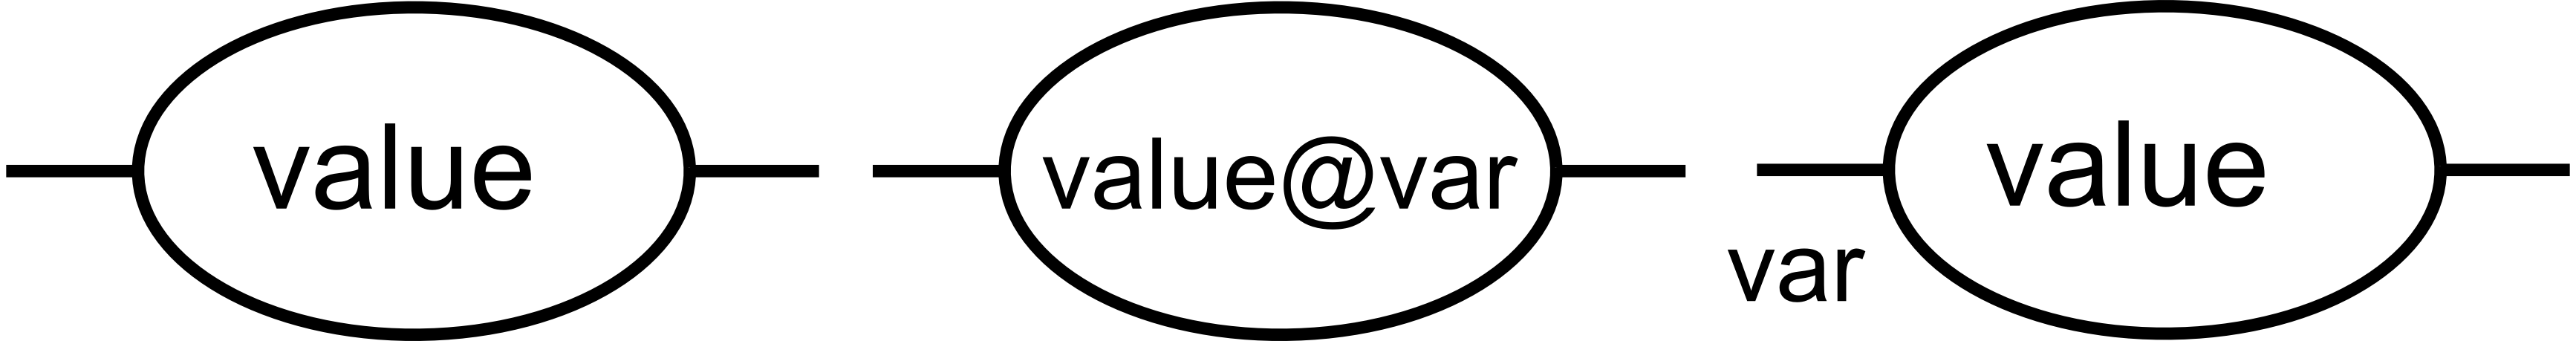
\includegraphics{images/stateVariable}
  \caption{The \PD glyph for \glyph{state variable}, shown with a value and a variable on the far left, with only a value on the middle-left, with an additional label for the variable on the middle-right (discouraged), and decorating a \glyph{macromolecule} (\sect{macromolecule}) on the far right.}
  \label{fig:state-var}
\end{figure}

\begin{figure}[H]
  \centering
    \begin{tabular}{lc}
        A & \raisebox{-\height}{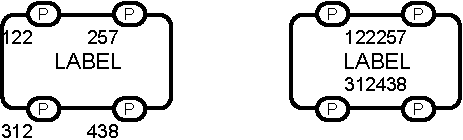
\includegraphics{examples/wrongStateVariablesA}}\\
        B & \raisebox{-\height}{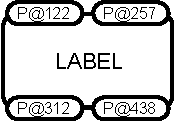
\includegraphics{examples/wrongStateVariablesB}}
    \end{tabular}
  \caption{A. Examples of discouraged use of \glyph{state variables}. B. Encouraged use.}
 \label{fig:wrong-state-var}
\end{figure}

% The following is for [X]Emacs users.  Please leave in place.
% Local Variables:
% TeX-master: "../sbgn_PD-level1"
% End:

 % FIX 101717
\subsection{Glyphs: \glyph{Clone markers}}
\label{sec:cloneMarker}

If an \glyph{EPN} is duplicated on a map, it is necessary to indicate this fact by using the \glyph{clone marker} auxiliary unit.
The purpose of this marker is to provide the reader with a visual indication that this node has been cloned, and that at least one other occurrence of the \glyph{EPN} can be found in the map (or in a submap; see \sect{submap}).
The clone marker takes two forms, simple and labelled, depending on whether the node being cloned can carry state variables (\ie whether it is a stateful EPN).
Note that an \glyph{EPN} belongs to a single compartment.
If two glyphs labelled ``X'' are located in two different compartments, such as an EPN labelled ``ATP'' in the cytosol, and another EPN labelled ``ATP'' in the mitochondrial lumen, they represent different \glyph{EPNs} and therefore do not need to be marked as cloned.

\subsubsection{\glyph{Simple clone marker}}

\begin{glyphDescription}

\glyphSboTerm
Not applicable.


\glyphIncoming
None.



\glyphOutgoing
None.


\glyphContainer
A \glyph{simple clone marker} is represented by a portion of the surface of an \glyph{EPN} that has been modified visually through the use of a different shade, texture, or colour, as shown in \fig{simpleCloneMarker}.
The \glyph{simple clone marker} occupies the lower part of the \glyph{EPN}.
The filled area must be smaller than the unfilled one.

\glyphLabel
None.

\glyphAux
None.

\end{glyphDescription}

\begin{figure}[H]
  \centering
  
\includegraphics{images/build/simple_clone_marker.pdf}
  \caption{The \PD glyph for \glyph{simple clone marker} applied to a \glyph{simple chemical} and a \glyph{multimer} of \glyph{simple chemicals}.}
  \label{fig:simpleCloneMarker}
\end{figure}

\fig{example-cloning} contains an example in which we illustrate the use of \glyph{simple clone markers} to clone the species ATP and ADP participating in different processes.  This example also demonstrates the chief drawbacks of using clones: it leads to a kind of dissociation of the overall network and multiplies the number of nodes required, requiring more work on the part of the reader to interpret the result.  Sometimes these disadvantages are offset in larger maps by a reduction in the overall number of line crossings, but not always.  In general, we advise that cloning should be used sparingly.

\begin{figure}[H]
  \centering
  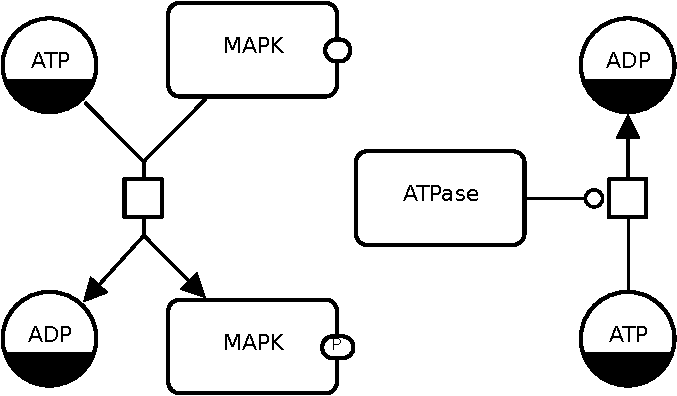
\includegraphics[scale = 0.8]{images/build/cloning_example.pdf}
  \caption{An example of using cloning, here for the species ATP and ADP.}
  \label{fig:example-cloning}
\end{figure}

\subsubsection{\glyph{Labelled clone marker}}

Unlike the \glyph{simple clone marker}, the \glyph{labelled clone marker} includes (unsurprisingly, given its name) an identifying label that can be used to identify equivalent clones elsewhere in the map.
This is particularly useful for stateful \glyph{EPNs} because these can have a large number of state variables displayed and therefore may be difficult to identify as being identical visually.
All duplicated stateful EPNs must be decorated with a \glyph{labelled clone marker}.

\begin{glyphDescription}

\glyphSboTerm Not applicable.


\glyphIncoming
None.



\glyphOutgoing
None.


\glyphContainer
The \glyph{labelled clone marker} is represented by a portion of the surface of an \glyph{EPN} that has been modified visually through the use of a different shade, texture, or colour, as shown in \fig{labelledCloneMarker}.
The \glyph{labelled clone marker} occupies the lower part of the \glyph{EPN}.
The filled area must be smaller than the unfilled one, but be large enough to accommodate the \glyph{labelled clone marker}'s label.

\glyphLabel
A \glyph{labelled clone marker} is identified by a label that is  a string of characters that may be distributed on several lines to improve readability.
The centre of the label must be placed on the centre of the container.
The label may extend outside of the container.
The font colour of the label and the colour of the \glyph{labelled clone marker} should contrast with one another.
The label on a \glyph{labelled clone marker} is mandatory.

\glyphAux
None.

\end{glyphDescription}

\begin{figure}[H]
  \centering
  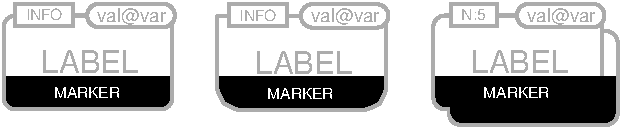
\includegraphics{images/build/labeled_clone_marker.pdf}
  \caption{The \PD glyph for \glyph{labelled clone marker} applied to a \glyph{macromolecule}, a \glyph{nucleic acid feature} and a \glyph{multimer} of \glyph{macromolecules}.}
  \label{fig:labelledCloneMarker}
\end{figure}

% The following is for [X]Emacs users.  Please leave in place.
% Local Variables:
% TeX-master: "../sbgn_PD-level1"
% End:
 % Done, Ugur
% $HeadURL$

%%%%%%%%%%%%%%%%%%%%%%%%%%%%%%%%%%%%%%%%%%%%%%%%%%%%%%%%%%%%%%%%%%%%%%
%%                     Subunit
%%%%%%%%%%%%%%%%%%%%%%%%%%%%%%%%%%%%%%%%%%%%%%%%%%%%%%%%%%%%%%%%%%%%%%

\subsection{Glyph\add{s}: \glyph{Subunits}}
\label{sec:subunit}

\corr{The \glyph{subunit} is used to describe the composition of the \glyph{complex}.
A \glyph{complex} can optionally be decorated with one or more subunits, which represent the types of \corr{\glyph{EPN}}{entities} that may aggregate to form a \glyph{complex}.
A \glyph{subunit} is an auxiliary unit that decorates the \glyph{complex} and does not represent or mimic an \glyph{EPN} directly, it only indicates the type of subunit included in the \glyph{complex}.
The example in \fig{complexSubunits} illustrates the use of \glyph{subunits} in a \glyph{complex}.
It also shows an equivalent complex without subunits.
}
{
A complex is formed by the non-covalent binding of two or more entities, that become the subunits of the complex.
In \PD, the composition of a complex may be described using \glyph{subunit} glyphs, that are auxiliary units decorating \glyph{complexes}.
\glyph{Subunits} do not represent or mimic entity pools~(\sect{EPNs}) and may only be used to represent the subunits included in a complex.
The example in \fig{complexSubunits} illustrates the use of \glyph{subunits} to describe the composition of a complex.
It also shows how the same complex can be represented without decorating \glyph{subunits}.
}

\add{
The SBGN \PD defines nine different \glyph{subunit} glyphs, each representing a different type of bio-molecular (sub)-entity.
The five main \glyph{subunits} are the \glyph{unspecified entity subunit}, \glyph{macromolecule subunit}, \glyph{simple chemical subunit}, \glyph{nucleic acid feature subunit}, and \glyph{complex subunit}.
\rougny{Maybe no need to list all subunits?}
This latter \glyph{subunit} allows representing complexes formed of other complexes.
The remaining four \glyph{subunits} are multimeric: \glyph{multimer of macromolecules subunit}, \glyph{multimer of simple chemicals subunit}, \glyph{multimer of nucleic acid feature subunit}, and \glyph{multimer of complexes subunit}.
}

\begin{glyphDescription}

\glyphSboTerm
Not applicable.

\add{
\glyphIncoming
None.
}

\add{
\glyphOutgoing
None.
}
\rougny{Is this true? No modulation arcs can depart from subunits inside complexes?
I'm pretty sure I've seen this in some maps though.}
% \corr{The symbol used for the}{The shape of used to represent a} \glyph{subunit} \corr{glyph}{} varies depending on the \glyph{subunit} type.
% The available \corr{symbols}{shapes} are equivalent to those used by the \glyph{EPN} glyphs (see \sect{EPNs})\add{,} including the \glyph{complex}.
% Therefore it is possible to describe complexes within complexes. The mapping between \corr{these and the symbol}{the \glyph{subunit} types and the containers to be used} is shown in the \tab{subunit_containers} below.
% }{
\glyphContainer
\add{Each \glyph{subunit} is represented by \corr{a different}{its own} shape depending on its bio-molecular nature, as shown in \tab{subunit_containers}.\blinov{Shapes may be identical.}
Those shapes are the same as those used to represent entity pools~(\sect{EPNs}).
\corr{However, \glyph{subunits} do not represent the same concepts, and can be seen as ``homonyms''.}{}}\blinov{Homonyms are never defined.}
% }

\luna{032819 replace string of characters with character string}
\corr{\glyphLabel A \glyph{subunit} is identified by a label that is \corr{an unbordered box containing}{} a string of characters \corr{.
The characters}{that} can be distributed on several lines to improve readability. \corr{, although this is not mandatory}{}.
The centre of the label box must be attached to the centre of the container.
The label may spill outside of the container.
}
{
\glyphLabel
A \glyph{subunit} is identified by a label that is \corr{an unbordered box containing}{} a string of characters \corr{.
The characters}{that} can be distributed on several lines to improve readability.
\dogrusoz{how about we simply say: "The characters may be distributed on several lines to improve readability." Not mandatory part is redundant I think.\\
AR: done for all glyphs}
The centre of the label must be placed on the centre of the \corr{shape}{container}.
The label may extend outside of the \corr{shape}{container}.
}


\add{\glyphAux A \glyph{subunit} may carry auxiliary units, depending on its type.}

\add{A \glyph{macromolecule}, \glyph{nucleic acid feature}, or \glyph{complex subunit} can carry one or more \glyph{state variables} that add information about its state (\sect{stateVariable}).
The state of such a \glyph{subunit} is defined as the set of all its \glyph{state variables}.}

\add{A \glyph{macromolecule}, \glyph{simple chemical}, \glyph{nucleic acid feature}, or \glyph{complex subunit} can carry one or more \glyph{units of information} (\sect{unitInfo}).
These can characterize a domain, such as a binding site.
Particular \glyph{units of information} are available for describing the material type (\sect{material-types-cv}) and conceptual type (\sect{conceptual-types-cv}) of such a \glyph{subunit}}.

\end{glyphDescription}

\begin{table}[h]
\begin{tabu}{X[c,m]X[c,m]X[c,m]X[c,m]}
    \toprule
    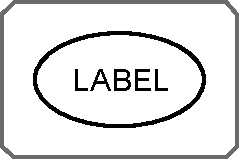
\includegraphics[scale = 0.8, valign = m]{images/unspecified-subunit} & 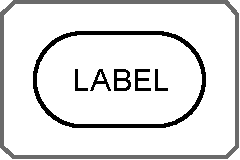
\includegraphics[scale = 0.8, valign = m]{images/simple_chemical-subunit} & 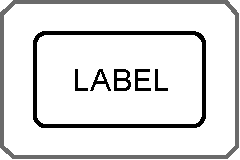
\includegraphics[scale = 0.8, valign = m]{images/macromolecule-subunit} & 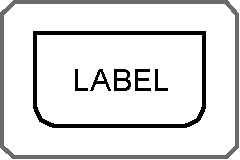
\includegraphics[scale = 0.8, valign = m]{images/genetic-subunit}\\[0.2cm]
    \glyph{unspecified entity subunit} & \glyph{simple chemical subunit} & \glyph{macromolecule subunit} & \glyph{nucleic acid feature subunit}\\[0.5cm]
    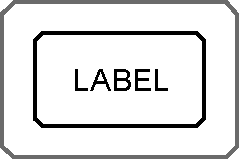
\includegraphics[scale = 0.8, valign = m]{images/complex-subunit} & 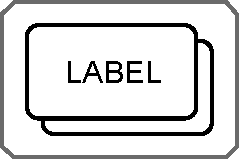
\includegraphics[scale = 0.8, valign = m]{images/macromolecule-multimer-subunit} & 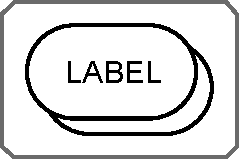
\includegraphics[scale = 0.8, valign = m]{images/simple_chemical-multimer-subunit} & 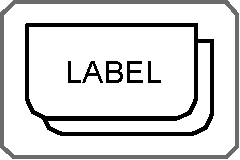
\includegraphics[scale = 0.8, valign = m]{images/genetic-multimer-subunit}\\[0.2cm]
    \glyph{complex subunit} & \glyph{multimer of macromolecules subunit} & \glyph{multimer of simple chemicals subunit} & \glyph{multimer of nucleic acid feature subunit}\\[0.5cm]
    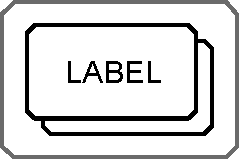
\includegraphics[scale = 0.8, valign = m]{images/complex-multimer-subunit} &  &  & \\[0.2cm]
    \glyph{multimer of complexes subunit} & & & \\
    \bottomrule
\end{tabu}
\caption{The \PD glyphs for the different types of \glyph{subunits}.
Each \glyph{subunit} decorates a \glyph{complex}.}
\label{tab:subunit_containers}
\end{table}


\begin{figure}[htb]
  \centering
  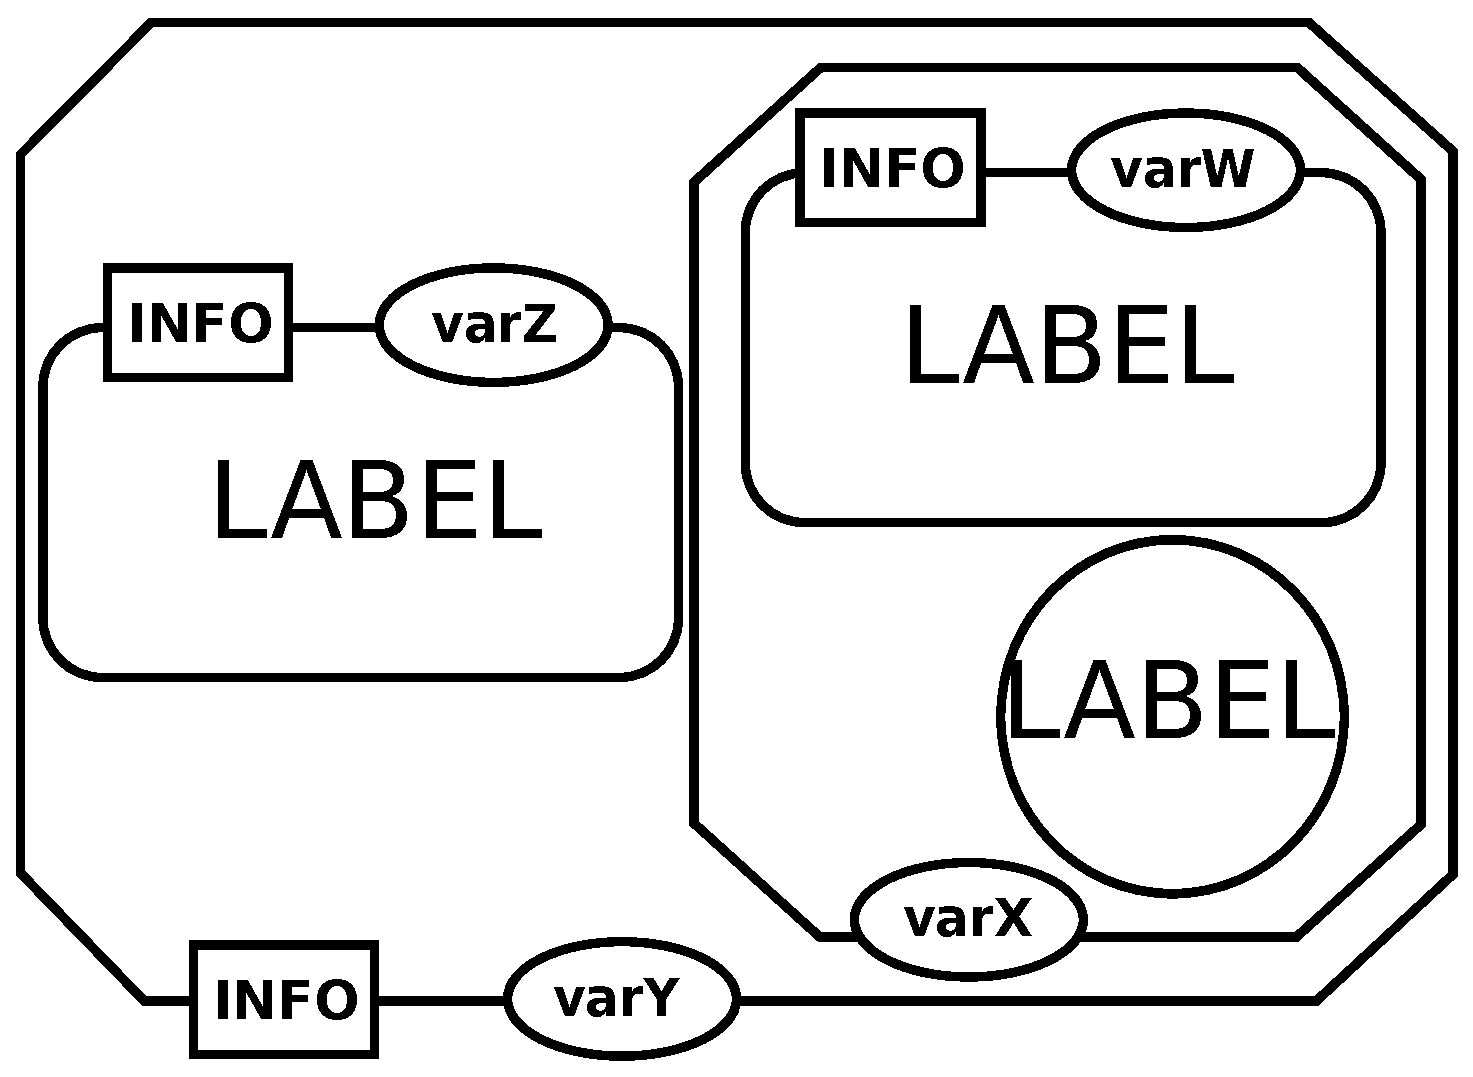
\includegraphics[scale=0.8]{images/complex}
  \caption{Both these complex glyphs are equivalent.
      The \corr{one}{complex} on the left is described using \glyph{subunit} decorators\corr{, the one}{.}
      \add{The complex} on the right depicts the same information, \corr{without them}{without explicitly representing those subunits, that are only suggested by the label of the \glyph{complex}.
  However, their states are represented using \glyph{state variables} decorating the \glyph{complex}.}}
  \label{fig:complexSubunits}
\end{figure}



\subsection{Glyph: \glyph{Submap terminal}}
\label{sec:submapTerminal}

A \glyph{submap teminal} is a decorator of the \glyph{submap} (\sect{submap}).
It is a named handle, or reference, to both an \glyph{EPN} (\sect{EPNs}) or \glyph{compartment} (\sect{compartment}) of the map, and a \glyph{tag} (\sect{tag}) of the map the \glyph{submap} glyph refers to.
Together with the \glyph{tag}, it allows linking glyphs of a map to their counterpart lying in a submap.

\begin{glyphDescription}

\glyphSboTerm Not applicable.

\glyphIncoming
One \glyph{equivalence arc} (\sect{equivalenceArc}).

\glyphOutgoing
None.

\glyphContainer A \glyph{submap terminal} is represented by a rectangular shape fused to an empty arrowhead, as shown in \fig{submapTerminal}.
The flat edge opposite to the arrowhead should be aligned to the edge of the \glyph{submap} glyph, and the incoming \glyph{equivalence arc} (\sect{equivalenceArc}) should be linked to its middle.

\glyphLabel A \glyph{submap terminal} is identified by a label that is  a string of characters that may be distributed on several lines to improve readability.
The centre of the label must be placed on the centre of the container.
The label may extend outside of the container.

\glyphAux
None.

\end{glyphDescription}

\begin{figure}[H]
  \centering
  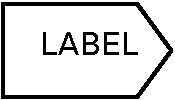
\includegraphics{images/build/submap_terminal.pdf}
  \caption{The \PD glyph for \glyph{submap terminal}.}
  \label{fig:submapTerminal}
\end{figure}



%%%%%%%%%%%%%%%%%%%%%%%%%%%%%%%%%%%%%%%%%%%%%%%%%%%%%%%%%%%%%%%%%%%%%%
%%%%%%%%%%%%%%%%%%%%%%%%%%%%%%%%%%%%%%%%%%%%%%%%%%%%%%%%%%%%%%%%%%%%%%
%%%%                   State nodes
%%%%%%%%%%%%%%%%%%%%%%%%%%%%%%%%%%%%%%%%%%%%%%%%%%%%%%%%%%%%%%%%%%%%%%
%%%%%%%%%%%%%%%%%%%%%%%%%%%%%%%%%%%%%%%%%%%%%%%%%%%%%%%%%%%%%%%%%%%%%%

\section{Entity pool nodes}\label{sec:EPNs}

An entity pool is a population of entities that cannot be distinguished from each other when it comes to the \SBGNPDLone map.
For instance, all the molecular  entities that fulfill the same role in a given process form an entity pool.
As a result, an entity pool can represent different granularity levels, such as all the proteins, all the instances of a given protein, only certain forms of a given protein.
To belong to a different compartment is sufficient to belong to different entity pools.
Calcium ions in the endoplasmic reticulum and calcium ions in the cytosol belong to different entity pools when it comes to representing calcium release from the endoplasmic reticulum.

The \PD contains six glyphs representing classes of material entities: \glyph{unspecified entity} (\sect{unspecifiedEntity}), \glyph{simple chemical} (\sect{simpleChemical}), \glyph{macromolecule} (\sect{macromolecule}), \glyph{nucleic acid feature} (\sect{genetic}), \glyph{multimer} (\sect{multimer}) and \glyph{complex} (\sect{complex}).
(Specific types of macromolecules, such as protein, RNA, DNA, polysaccharide, and specific simple chemicals are not defined by \PD but may be part of future levels of SBGN.)
In addition to the material entities, \PD represents two conceptual entity pools: \glyph{empty set} (\sect{emptySet}), and \glyph{perturbing agent} (\sect{perturbing agent}).
Material and conceptual entities can optionally carry auxiliary units such as \glyph{units of information} (\sect{unitInfo}), \glyph{state variables}  (\sect{stateVariable}) and \glyph{clone markers} (\sect{cloneMarker}).

% $HeadURL$

\subsection{Glyph: \glyph{Unspecified entity}}
\label{sec:unspecifiedEntity}

The simplest type of EPN is the \glyph{unspecified entity}: one whose type is unknown or simply not relevant to the purposes of the map.
This arises, for example, when the existence of the entity has been inferred indirectly, or when the entity is merely a construct introduced for the needs of a map, without direct biological relevance.
These are examples of situations where the \emph{unspecified entity} glyph is appropriate.
(Conversely, for cases where the identity of the entities composing the pool is known, there exist other, more specific glyphs described elsewhere in the specification.)

\begin{glyphDescription}

\glyphSboTerm
 SBO:0000285 ! material entity of unspecified nature


\glyphIncoming
Zero or more \glyph{production} arcs (\sect{production}).



\glyphOutgoing
Zero or more \glyph{consumption} arcs (\sect{consumption}), \glyph{modulation arcs} (\sect{modulations}), \glyph{logic arcs} (\sect{logicArc}), or \glyph{equivalence arcs} (\sect{equivalenceArc}).


\glyphContainer
A \glyph{unspecified entity} is represented by an elliptic shape, as shown in \fig{unspecified}.
Note that the shape must remain an ellipse to avoid confusion with \glyph{simple chemical}, which is represented with a stadium shape (\sect{simpleChemical}).

\glyphLabel
A \glyph{unspecified entity} is identified by a label  that is a string of characters that may be distributed on several lines to improve readability.
The centre of the label must be placed on the centre of the container.
The label may extend outside of the container.



\glyphAux
An \glyph{unspecified entity} can carry a \glyph{clone marker} (see \sect{cloneMarker}).

\end{glyphDescription}

\begin{figure}[H]
  \centering
  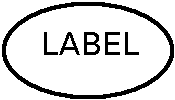
\includegraphics{images/build/unspecified.pdf}
  \caption{The \PD glyph for \glyph{unspecified entity}.}
  \label{fig:unspecified}
\end{figure}

% The following is for [X]Emacs users.   Please leave in place.
% Local Variables:
% TeX-master: "../sbgn_PD-level1"
% End:

\subsection{Glyph: \glyph{Simple chemical}}
\label{sec:simpleChemical}

A simple chemical in SBGN is defined as the opposite of a macromolecule (\sect{macromolecule}): it is a chemical compound that is \emph{not} formed by the covalent linking of pseudo-identical residues. \borlinghaus{Here we first describe the opposite of a macromolecule using the definition of a macromolecule that is explained later. Would it make sense to change the order here?}
Examples \corr{of simple chemicals}{} are an atom, a monoatomic ion, a salt, a radical, a solid metal, a crystal, etc.

\begin{glyphDescription}

\glyphSboTerm
SBO:0000247 ! simple chemical

\add{
\glyphIncoming
Zero or more \glyph{production} arcs (\sect{production}).
}

\add{
\glyphOutgoing
Zero or more \glyph{consumption} arcs (\sect{consumption}), \glyph{modulation arcs} (\sect{modulations}), \glyph{logic arcs} (\sect{logicArc}), or \glyph{equivalence arcs} (\sect{equivalenceArc}).
}

\glyphContainer
A \glyph{simple chemical} is represented by a ``stadium'' shape, that is two semicircles of the same radius joined by parallel line segments, as shown in \fig{simpleChemical}.
If desired the parallel line segments can have zero length, and the shape is then identical to a circle.
To avoid confusion with the \glyph{unspecified entity} (\ref{sec:unspecifiedEntity}), this form of the glyph must remain a circle and cannot be deformed into an ellipse.
\glyphLabel
A \glyph{simple chemical} is identified by a label \corr{an unbordered box containing}{} that is a string of characters \corr{.
The characters}{that} may be distributed on several lines to improve readability.
The centre of the label must be placed on the centre of the \corr{shape}{container}.


\glyphAux
A \glyph{simple chemical} can carry one or more \glyph{units of information} (\sect{unitInfo}).
% These can characterise <EXAMPLES>.
Particular \glyph{units of information} are available for describing the material type (\sect{material-types-cv}) and the conceptual type (\sect{conceptual-types-cv}) of a \glyph{simple chemical}.

A \glyph{simple chemical} can also carry a \glyph{simple clone marker} (see \sect{cloneMarker}).

\end{glyphDescription}

\begin{figure}[H]
  \centering
  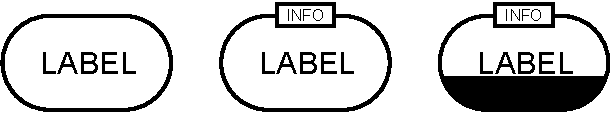
\includegraphics{images/simple_chemical-combined}
  \caption{The \PD glyph for a \glyph{simple chemical}, shown plain and unadorned on the left, with an additional \glyph{unit of information} in the middle, and with a \glyph{simple clone marker} on the right.}
  \label{fig:simpleChemical}
\end{figure}

% The following is for [X]Emacs users.  Please leave in place.
% Local Variables:
% TeX-master: "../sbgn_PD-level1"
% End:

% $HeadURL: https://sbgn.svn.sourceforge.net/svnroot/sbgn/ProcessDiagram/tags/L1V1.3Full/sources/macromolecule.tex $

\subsection{Glyph: \glyph{Macromolecule}}
\label{sec:macromolecule}

Many biological processes involve \emph{macromolecules}: biochemical substances that are built up from the covalent linking of pseudo-identical units.  Examples of macromolecules include proteins, nucleic acids (RNA, DNA), and polysaccharides (glycogen, cellulose, starch, etc.).  Attempting to define a separate glyph for all of these different molecules would lead to an explosion of symbols in SBGN, so instead, \SBGNPDLone defines only one glyph for all macromolecules.  The same glyph is to be used for a protein, a nucleic acid, a complex sugar, and so on.  The exact nature of a particular macromolecule in a map is then clarified using its label and decorations, as will become clear below.  A \glyph{macromolecule} is represented by a rectangular container with rounded corners, as illustrated in \fig{macromolecule}. 

\begin{figure}[H]
  \centering
  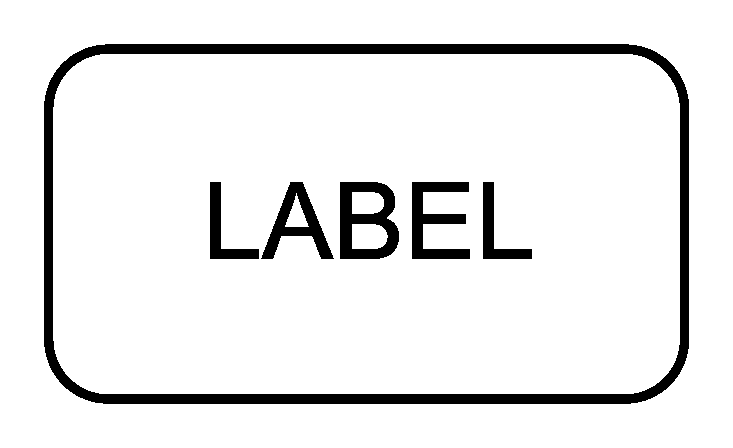
\includegraphics[width = 1.25in]{images/macromolecule-plain}
  \caption{The \PD glyph for \glyph{macromolecule}.}
  \label{fig:macromolecule}
\end{figure}

Examples of \glyph{macromolecules} are presented in \fig{macromolecule-examples}.

\begin{figure}[H]
  \centering
  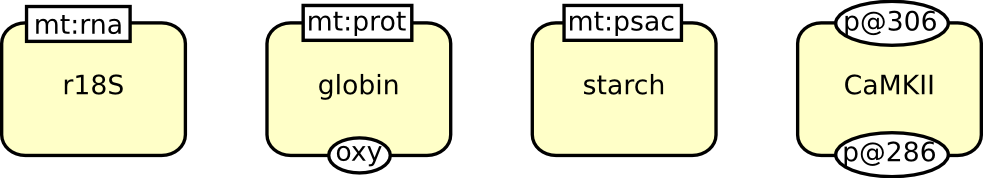
\includegraphics[scale = 0.5]{images/macromolecule-examples}
  \caption{Examples of \glyph{macromolecules}. From left to right: the macromolecule of 18S ribosomal RNA, globin (a protein) in the oxygenated state, a molecule of starch (polymer of glucose), calcium calmodulin kinase 2 phosphorylated on threonine 286 and 306.}
  \label{fig:macromolecule-examples}
\end{figure}




% The following is for [X]Emacs users.   Please leave in place.
% Local Variables:
% TeX-master: "../sbgn_PD-level1"
% End:
 % FIX 101717
% $HeadURL$

\subsection{Glyph: \glyph{Nucleic acid feature}}
\label{sec:genetic}

The \emph{nucleic acid feature} represents a fragment of a macromolecule carrying genetic information.
A common use for this construct is to represent a gene or transcript.
The label of this EPN and its \emph{units of information} are often crucial for making the purpose clear to the reader of a map.

\begin{glyphDescription}

\glyphSboTerm
SBO:0000354 ! informational molecule segment


\glyphIncoming
Zero or more \glyph{production} arcs (\sect{production}).



\glyphOutgoing
Zero or more \glyph{consumption} arcs (\sect{consumption}), \glyph{modulation arcs} (\sect{modulations}), \glyph{logic arcs} (\sect{logicArc}), or \glyph{equivalence arcs} (\sect{equivalenceArc}).


\glyphContainer
A \glyph{nucleic acid feature} is represented by a rectangular shape whose bottom half has rounded corners.
This design reminds us that we are fundamentally dealing with a unit of information carried by a macromolecule.

\glyphLabel
A \glyph{nucleic acid feature} is identified by a label that is  a string of characters that may be distributed on several lines to improve readability.
The centre of the label must be placed on the centre of the container.
The label may extend outside of the container.

\glyphAux
A \glyph{nucleic acid feature} can carry one or more \glyph{state variables} that add information about its state (\sect{stateVariable}).
The state of a \glyph{nucleic acid feature} is defined as the set of all its \glyph{state variables}.

A \glyph{nucleic acid feature} can also carry one or more \glyph{units of information} (\sect{unitInfo}).
These can characterise a domain, such as a binding site.
Particular \glyph{units of information} are available for describing the material type (\sect{material-types-cv}) and the conceptual type (\sect{conceptual-types-cv}) of a \glyph{nucleic acid feature}.

Finally, a \glyph{nucleic acid feature} can also carry a \glyph{labelled clone marker} (see \sect{cloneMarker}).

\end{glyphDescription}

\begin{figure}[H]
  \centering
  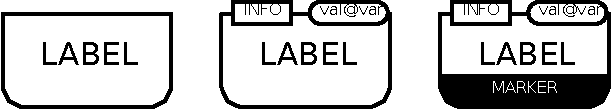
\includegraphics{images/build/genetic_combined}% \hspace*{2em.pdf}
  %\raisebox{0.04in}{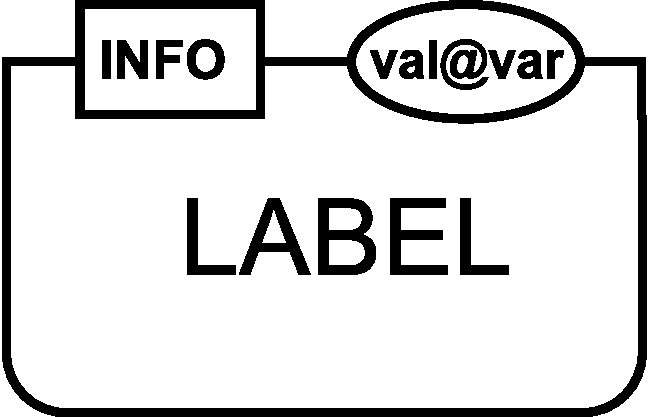
\includegraphics[width = 1.25in]{images/build/genetic}.pdf}
  \caption{The \PD glyph for \glyph{nucleic acid feature}, shown plain and unadorned on the left, with an additional \glyph{state variable} and a \glyph{unit of information} in the middle, and with a \glyph{labelled clone marker} on the right.}
  \label{fig:genetic}
\end{figure}

% The following is for [X]Emacs users.  Please leave in place.
% Local Variables:
% TeX-master: "../sbgn_PD-level1"

\subsection{Glyph: \glyph{Multimer}}
\label{sec:multimer}

As its name implies, a multimer is an aggregation of multiple identical or pseudo-identical entities held together by non-covalent bonds (thus, they are distinguished from polymers by the fact that the later involve covalent bonds).
Here,  \emph{pseudo-identical} refers to the possibility that the entities differ chemically but retain some common global characteristic, such as a structure or function, and so can be considered identical within the context of the SBGN \PD.
An example of this is the homologous subunits in a hetero-oligomeric receptor.

SBGN \PD defines four different \glyph{multimer} glyphs: \glyph{simple chemical multimer}, \glyph{macromolecule multimer}, \glyph{nucleic acid feature multimer} and \glyph{complex multimer}.



\begin{glyphDescription}

\glyphSboTerm
\begin{tabular}{l l}
    & SBO:0000286 ! multimer\\
\glyph{Simple chemical multimer} & SBO:0000421 ! multimer of simple chemicals\\
\glyph{Macromolecule multimer} & SBO:0000420 ! multimer of macromolecules \\
\glyph{Complex multimer} & SBO:0000418 ! multimer of complexes \\
\glyph{Nucleic acid feature multimer} & SBO:0000419 ! multimer of informational molecule segments \\
\end{tabular}


\glyphIncoming
Zero or more \glyph{production} arcs (\sect{production}).



\glyphOutgoing
Zero or more \glyph{consumption} arcs (\sect{consumption}), \glyph{modulation arcs} (\sect{modulations}), \glyph{logic arcs} (\sect{logicArc}), or \glyph{equivalence arcs} (\sect{equivalenceArc}).



\glyphContainer
Each \glyph{multimer} is represented by a different shape depending on the bio-molecular nature of its pseudo-identical subunits, as shown in \tab{multimer_containers}.
The shape of a \glyph{multimer} consists of two \glyph{subunits} or \glyph{EPNs} shapes shifted horizontally and vertically, and stacked on top of another.




\glyphLabel
A \glyph{subunit} is identified by a label that is   a string of characters that may be distributed on several lines to improve readability.
% 
The centre of the label must be placed on the centre of the shape.
The label may extend outside of the shape.
The label should refer to the pseudo-identical subunits, and not to the multimer itself.



\glyphAux A \glyph{multimer} may carry auxiliary units, depending on its type.

A \glyph{macromolecule}, \glyph{nucleic acid feature}, or \glyph{complex multimer} can carry one or more \glyph{state variables} that add information about its state (\sect{stateVariable}).
The state of such a \glyph{multimer} is defined as the set of all its \glyph{state variables}.

A \glyph{multimer} of any type can carry one or more \glyph{units of information} (\sect{unitInfo}).
These can characterize a domain, such as a binding site.
Particular \glyph{units of information} are available for describing the material type (\sect{material-types-cv}), conceptual type (\sect{conceptual-types-cv}) and the cardinality (\sect{cardinality-cv}) of such a \glyph{multimer}.

Note that a \glyph{state variable} or a \glyph{unit of information} carried by a \glyph{multimer} actually applies to each of the subunits individually.
If instead the \glyph{state variables} or the \glyph{units of information} are meant to apply to the whole multimeric assembly, a \glyph{macromolecule} (\sect{macromolecule}) or a \glyph{complex} (\sect{complex}) should be used instead of a \glyph{multimer}.
An assembly containing some \glyph{state variables} or \glyph{units of information} applicable to the subunits, and other \glyph{state variables} or \glyph{units of information} applicable to the assembly (for instance opening of a channel and phosphorylation of each of its subunits) should be represented by a \glyph{complex} (\sect{complex}).

Finally, a \glyph{simple chemical multimer} can also carry a \glyph{simple clone marker} (\sect{cloneMarker}), and a \glyph{macromolecule}, \glyph{nucleic acid feature} or \glyph{complex multimer} a \glyph{labelled clone marker} (\sect{cloneMarker}).

\end{glyphDescription}

\begin{table}[h]
\begin{tabu}{X[c,m]X[c,m]X[c,m]X[c,m]}
    \toprule
    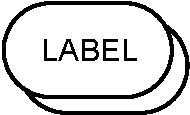
\includegraphics[valign = m]{images/simple_chemical-multimer} & 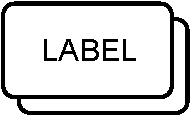
\includegraphics[valign = m]{images/macromolecule-multimer} & 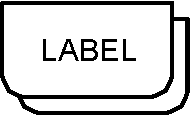
\includegraphics[valign = m]{images/genetic-multimer} & 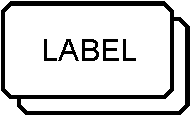
\includegraphics[valign = m]{images/complex-multimer}\\[0.5cm]
    \glyph{simple chemical multimer} & \glyph{macromolecule multimer} & \glyph{nucleic acid feature multimer} & \glyph{complex multimer}\\
	\bottomrule
\end{tabu}
\caption{The \PD glyphs for the different types of \glyph{multimers}.}
\label{tab:multimer_containers}
\end{table}

% \begin{figure}[H]
%   \centering
%   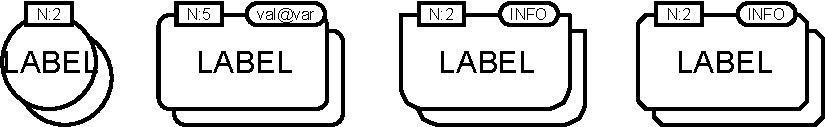
\includegraphics[scale = 0.3]{images/multimer}
%   \caption{The \PD glyph for \glyph{multimer} with an additional unit of information containing the cardinality.}
%   \label{fig:multimer}
% \end{figure}
% 

% The following is for [X]Emacs users.  Please leave in place.
% Local Variables:
% TeX-master: "../sbgn_PD-level1"
% End:

% $HeadURL$

%%%%%%%%%%%%%%%%%%%%%%%%%%%%%%%%%%%%%%%%%%%%%%%%%%%%%%%%%%%%%%%%%%%%%%
%%%%                   Complex
%%%%%%%%%%%%%%%%%%%%%%%%%%%%%%%%%%%%%%%%%%%%%%%%%%%%%%%%%%%%%%%%%%%%%%

\subsection{Glyph: \glyph{Complex}}\label{sec:complex}

A \glyph{complex} represents a pool of biochemical entities, each composed of other biochemical entities, whether macromolecules, simple chemicals, multimers, or other complexes. The resulting entity may have its own identity, properties and function in an SBGN map.
The \glyph{complex} can be described by the set of \glyph{subunits} \add{(\sect{subunit})} it contains (see \fig{complexSubunits}). This description is entirely optional and is there to assist the user with a visual shorthand about the composition of the complex.
% \rougny{Chaneg first sentence to ``A complex represents a pool if biochemical entities, each composed of other biochemical entities...''?}

\begin{glyphDescription}

\glyphSboTerm
SBO:0000253 ! non-covalent complex

\add{
\glyphIncoming
Zero or more \glyph{production} arcs (\sect{production}).
}

\add{
\glyphOutgoing
Zero or more \glyph{consumption} arcs (\sect{consumption}), \glyph{modulation arcs} (\sect{modulations}), \glyph{logic arcs} (\sect{logicArc}), or \glyph{equivalence arcs} (\sect{equivalenceArc}).
}

\glyphContainer
\corr{A \glyph{complex} possesses its own container box surrounding the juxtaposed container boxes of its components.
This container box is a rectangle with cut-corners (an octagonal box with sides of two different lengths). The size of the cut-corners are adjusted so that there is no overlap between the container and the components. The container boxes of the components must not overlap.}{
A \glyph{complex} is represented by a rectangular shape with cut-corners (that is, an octogonal shape with sides of two different lengths).
If the \glyph{complex} is described by a set of \glyph{subunits}, then its shape should surround those of its \glyph{subunits}, and the size of the cut-corners should be adjusted so that there is no overlap between its shape and those of its \glyph{subunits}.
The shapes of the \glyph{subunits} must not overlap.}

\glyphLabel
A \glyph{complex} is identified by a label that is \corr{an unbordered box containing}{} a string of characters \corr{.
The characters}{that} may be distributed on several lines to improve readability\corr{, although this is not mandatory}.
\corr{Ideally, the label box should be attached to the midway between the border of the complex's container box and the border of the components' container boxes. However, if the \glyph{complex} contains \glyph{subunits} glyphs then the label may be positioned to optimise the clarity and avoid overlapping.}{
In the case where the \glyph{complex} is not described by a set of \glyph{subunits}, the centre of the label must be placed on the centre of the \glyph{complex}'s shape.
In the case where the \glyph{complex} is described by a set of \glyph{subunits}, the label may be positioned to optimize the clarity and avoid overlapping, ideally between the bottom-most or the upper-most \glyph{subunit} and the border of the \glyph{complex}.
}

\glyphAux
A \glyph{complex} can carry one or more \glyph{state variables} that add information about its state (\sect{stateVariable}).
\corr{The state of a \glyph{complex} is defined as the set of all its \glyph{state variables}}{} \corr{and all the state variables of all its components}{}.\rougny{In old v2, the state of a complex is only defined by its state variables, not additionally by those of its subunits} \blinov{Talking about the state of a complex is confusing.}

A \glyph{complex} can also carry one or more \glyph{units of information} (\sect{unitInfo}).
These can characterise a domain, such as a binding site.
Particular \glyph{units of information} are available for describing the material type (\sect{material-types-cv}) and the conceptual type (\sect{conceptual-types-cv}) of a \glyph{complex}.

Finally, a \glyph{complex} can also carry a \glyph{labelled clone marker} (see \sect{cloneMarker}).

\end{glyphDescription}

\begin{figure}[H]
  \centering
  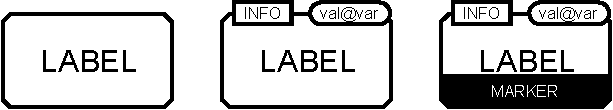
\includegraphics{images/complex-combined}
  \caption{The \PD glyph for \glyph{complex}, shown plain and unadorned on the left, with an additional \glyph{state variable} and a \glyph{unit of information} in the middle, and with a \glyph{labelled clone marker} on the right.}
  \label{fig:complex}
\end{figure}

% The following is for [X]Emacs users.  Please leave in place.
% Local Variables:
% TeX-master: "../sbgn_PD-level1"
% End:


\subsection{Glyph: \glyph{Empty Set}}
\label{sec:emptySet}

It is useful to have the ability to represent the creation of an entity or a state from an unspecified source, that is, from something that one does not need or wish to make precise.  For instance, in a model where the production of a protein is represented, it may not be desirable to represent all of the amino acids, sugars and other metabolites used, or the energy involved in the protein's creation.
Similarly, we may not wish to bother representing the details of the destruction or decomposition of some biochemical species into a large number of more primitive entities, preferring instead to simply say that the species ``disappears into a sink''.
Yet another example is that one may need to represent an input (respectively, output) into (respectively, from) a compartment without explicitly representing a transport process from a source (respectively, to a target).

For these and other situations, SBGN defines a single glyph representing the involvement of an external pool of entities.
The symbol used in SBGN is borrowed from the mathematical symbol for ``empty set'', but it is important to note that it does not actually represent a true absence of everything or a physical void---it represents the absence of the corresponding structures in the model, that is, the fact that the external pool is conceptually outside the scope of the map.

A frequently asked question is, why bother having an explicit symbol at all?
The reason is that one cannot simply use an arc that does not terminate on a node, because the dangling end could be mistaken to be pointing to another node in the map.  This is specially true if the map is rescaled, causing the spacing of elements in the map to change.
The availability and use of an explicit symbol for sources and sinks is crucial.

\begin{glyphDescription}

\glyphSboTerm
SBO:0000291 ! empty set

\add{
\glyphIncoming
Zero or one \glyph{production} arcs (\sect{production}).
}

\add{
\glyphOutgoing
Zero or one \glyph{consumption} arcs (\sect{consumption}).
}

\glyphContainer
An \glyph{empty set} is represented by a circular shape crossed by a bar linking the lower-left and upper-right corners of the circle's bounding box, as shown in \fig{emptySet}.

\glyphLabel
None.

\glyphAux
None.

\end{glyphDescription}

\begin{figure}[H]
  \centering
  
\includegraphics{images/emptySet}
  \caption{The \PD glyph for \glyph{empty set}.}
  \label{fig:emptySet}
\end{figure}

% The following is for [X]Emacs users.    Please leave in place.
% Local Variables:
% TeX-master: "../sbgn_PD-level1"
% End:

% $HeadURL$

\subsection{Glyph: \glyph{Perturbing agent}}
\label{sec:perturbing agent}

Biochemical networks can be affected by external influences.
Those influences can be the effect of well-defined physical perturbing agents, such as a light pulse or a change in temperature; they can also be more complex and not well-defined phenomena, for instance the outcome of a biological process, an experimental setup, or a mutation.
For these situations, \PD provides the \glyph{perturbing agent} glyph. It is an EPN, and represents the amount of perturbing agent applied to a process.

\begin{glyphDescription}

\glyphSboTerm
SBO:0000405 ! perturbing agent

\add{
\glyphIncoming
None.
}

\add{
\glyphOutgoing
One or more \glyph{modulation arcs} (\sect{modulations}) or \glyph{logic arcs} (\sect{logicArc}), zero or more \glyph{equivalence arcs} (\sect{equivalenceArc}).
}

\glyphContainer
A \glyph{perturbing agent} is represented by a by a modified hexagonal shape having two opposite concave faces, as shown in \fig{perturbing_agent}.

\glyphLabel
A \glyph{perturbing agent} is identified by a label that is \corr{an unbordered box containing}{} a string of characters \corr{.
The characters}{that} may be distributed on several lines to improve readability.
The centre of the label must be placed on the centre of the \corr{shape}{container}.
The label may extend outside of the \corr{shape}{container}.

\glyphAux
A \glyph{perturbing agent} can carry one or more \glyph{units of information} (\sect{unitInfo}).
% These can characterise <EXAMPLES>.
Particular \glyph{units of information} are available for describing the material type (\sect{material-types-cv}) and the conceptual type (\sect{conceptual-types-cv}) of a \glyph{perturbing agent}, as well as its physical characteristic (see \sect{physical-characteristics-cv}).

A \glyph{perturbing agent} can also carry a \glyph{simple clone marker} (see \sect{cloneMarker}).

\end{glyphDescription}

\begin{figure}[H]
  \centering
  
\includegraphics{images/perturbing_agent}
  \caption{The \PD glyph for \glyph{perturbing agent}.}
  \label{fig:perturbing_agent}
\end{figure}

% The following is for [X]Emacs users.  Please leave in place.
% Local Variables:
% TeX-master: "../sbgn_PD-level1"
% End:



% $HeadURL$

\subsection{Examples of complex EPNs}
\label{sec:CplxEPNs}

In this section, we provide examples of Entity Pool Node representations drawn using the \SBGNPDLone glyphs described above. 

\fig{example-camkii} represents a pool of calcium/calmodulin kinase II entities, each with phosphorylation on the sites threonine 286 and 306, as well as catalytic and autoinhibitory domains.  Note the use of \emph{units of information} and \emph{state variables}.

\begin{figure}[H]
  \centering
  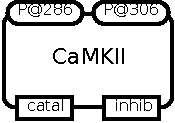
\includegraphics[scale = 0.8]{images/build/macromolecule_camkii_example.pdf}
  \caption{An example representation of calcium/calmodulin kinase II EPN.}
  \label{fig:example-camkii}
\end{figure}

\fig{example-glur} represents the glutamate receptor in the open state, with both phosphorylation and glycosylation.  The entity carries two functional domains, the ligand-binding domain and the ion pore, and its chemical nature is presided.

\begin{figure}[H]
  \centering
  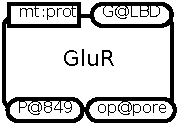
\includegraphics[scale = 0.8]{images/build/macromolecule_glu_r_example.pdf}
  \caption{An example of a glutamate receptor in the open state.}
  \label{fig:example-glur}
\end{figure}

%%% Local Variables: 
%%% mode: latex
%%% TeX-master: "../sbgn_PD-level1"
%%% End: 


%%%%%%%%%%%%%%%%%%%%%%%%%%%%%%%%%%%%%%%%%%%%%%%%%%%%%%%%%%%%%%%%%%%%%%
%%%%%%%%%%%%%%%%%%%%%%%%%%%%%%%%%%%%%%%%%%%%%%%%%%%%%%%%%%%%%%%%%%%%%%
%%%%                   Containers
%%%%%%%%%%%%%%%%%%%%%%%%%%%%%%%%%%%%%%%%%%%%%%%%%%%%%%%%%%%%%%%%%%%%%%
%%%%%%%%%%%%%%%%%%%%%%%%%%%%%%%%%%%%%%%%%%%%%%%%%%%%%%%%%%%%%%%%%%%%%%

%\section{Container nodes}\label{sec:CNs}
\section{Defined sets of entity pool nodes}

\subsection{Glyph: \glyph{Compartment}}
\label{sec:compartment}

A compartment is a logical or physical structure that contains entity pool nodes. An EPN can only belong to one compartment. Therefore, the ``same'' biochemical species located in two different compartments are in fact two different pools.

\begin{glyphDescription}

\glyphSboTerm  SBO:0000290 ! physical compartment


\glyphIncoming
None.



\glyphOutgoing
Zero or more \glyph{equivalence arcs} (\sect{equivalenceArc}).


\glyphContainer
A \glyph{compartment} is represented by a surface enclosed in a continuous border or located between continuous borders.
These borders should be noticeably thicker than the borders of the EPNs.
A compartment can take \textbf{any} shape.
A compartment must always be entirely enclosed.

\glyphLabel
A \glyph{compartment} is identified by a label that is  a string of characters that may be distributed on several lines to improve readability.
The label can be placed anywhere in the shape.
The label may extend outside of the shape.

\glyphAux
A \glyph{compartment} can carry one or more \glyph{units of information} (\sect{unitInfo}).
These can characterise the physical environment, such as pH, temperature or voltage.




\end{glyphDescription}

\begin{figure}[H]
  \centering
  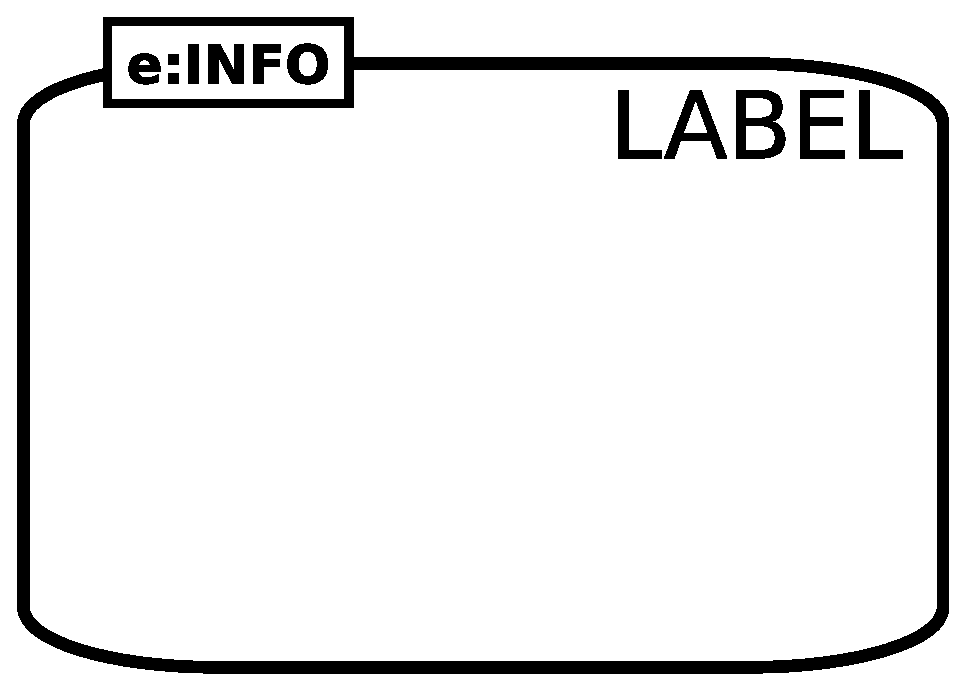
\includegraphics{images/compartment}
  \caption{The \PD glyph for \glyph{compartment}.}
  \label{fig:compartment}
\end{figure}

To allow more aesthetically pleasing and understandable maps, compartments are allowed to overlap each other visually, but it must be kept in mind that this does not mean the top compartment contains part of the bottom compartment.
\fig{overlap} shows two semantically equivalent placement of compartments:

\begin{figure}[H]
  \centering
  \includegraphics[scale = 0.5]{examples/compartment_overlapping}
  \caption{Overlapped compartments are permitted, but the overlap does not imply containment.}
  \label{fig:overlap}
\end{figure}

Overlapped (hidden) part of the compartment should not contain any object which could be covered by an overlapping compartment.
\fig{overlap-bad} illustrates the problem using an incorrect map.

\begin{figure}[H]
  \centering
  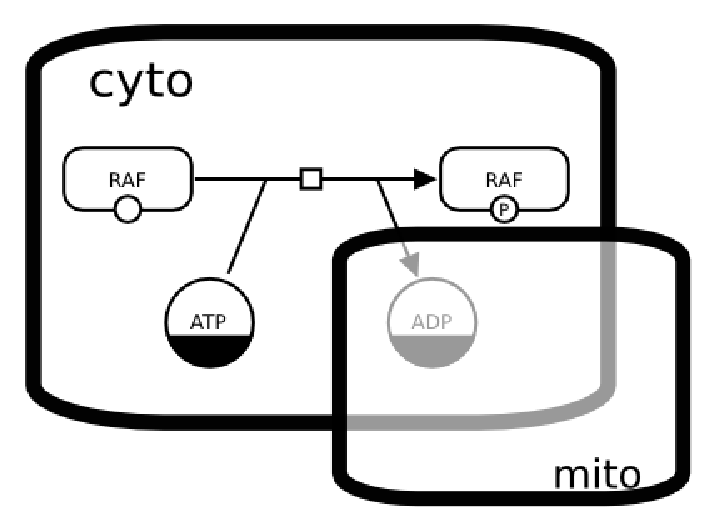
\includegraphics[scale = 0.8]{examples/compartment_overlapping_wrong}
  \caption{Example of an \textbf{incorrect} map.  Overlapped compartments must not obscure other objects.}
  \label{fig:overlap-bad}
\end{figure}

% It is important to note that a compartment never contains another compartment, but may surround it.  A key aspect of correctly drawing two ``adjacent'' compartments is that they are not separated by one line, but by \textbf{two} lines.  \fig{two-comp} provides an example of this in which a cell is shown made up of a nucleus surrounded by the cytoplasm.

% \begin{figure}[H]
%   \centering
%   \includegraphics[scale = 0.4]{examples/compartment-cell}
%  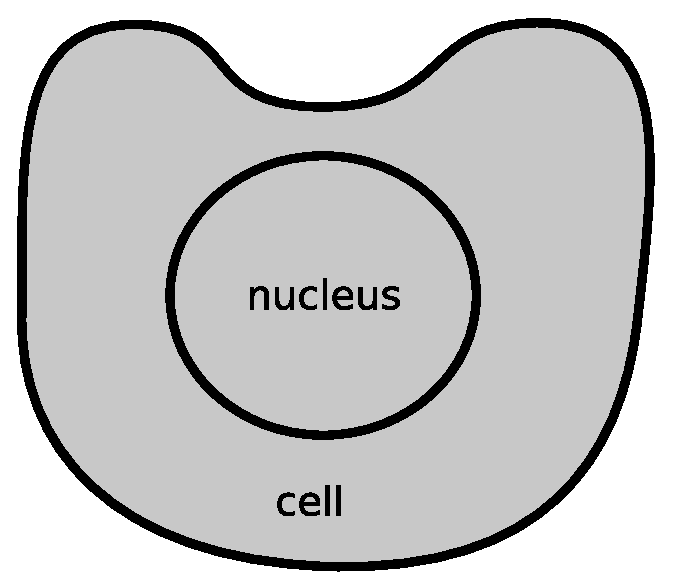
\includegraphics[scale = 0.4]{examples/compartment-cell-wrong}
%   \caption{Compartments can surround other compartments; in that case, both of the compartment's borders must still be shown, with the result that the separation is drawn as two lines. The left example is correct, with twoo disjoint compartments representing the ``cytoplasm'' and the ``nucleus''. The right example is incorrect. Indeed the compartments ``cell'' and ``nucleus'' would be disjoint, the latter only overlapping the former. As a result, the volume of the nucleus is duplicated.}
%   \label{fig:two-comp}
% \end{figure}

% The example diagram in \fig{three-comp} represents three adjacent compartments.  Two of the compartments carry units of information.  Notice that these units of information do not overlap multiple membrane boundaries.

% \begin{figure}[H]
%   \centering
%   \includegraphics[scale = 0.4]{examples/compartment-3comp}
%   \caption{Illustration of units of information and surrounding compartments.}
%   \label{fig:three-comp}
% \end{figure}

% The following is for [X]Emacs users.  Please leave in place.
% Local Variables:
% TeX-master: "../sbgn_PD-level1"
% End:


%%%%%%%%%%%%%%%%%%%%%%%%%%%%%%%%%%%%%%%%%%%%%%%%%%%%%%%%%%%%%%%%%%%%%%
%%%%%%%%%%%%%%%%%%%%%%%%%%%%%%%%%%%%%%%%%%%%%%%%%%%%%%%%%%%%%%%%%%%%%%
%%%%                   Process nodes
%%%%%%%%%%%%%%%%%%%%%%%%%%%%%%%%%%%%%%%%%%%%%%%%%%%%%%%%%%%%%%%%%%%%%%
%%%%%%%%%%%%%%%%%%%%%%%%%%%%%%%%%%%%%%%%%%%%%%%%%%%%%%%%%%%%%%%%%%%%%%

\section{Process nodes}\label{sec:PNs}

Process nodes represent processes that transform one or several entity pools into one or several entity pools, identical or different.  \SBGNPDLone defines a generic \glyph{process} (\sect{process}), as well as five more specific ones: the \glyph{omitted process} (\sect{omitted}), the \glyph{uncertain process} (\sect{uncertain}), the \glyph{association} (\sect{association}), the \glyph{dissociation} (\sect{dissociation}), and the \glyph{phenotype} (\sect{phenotype}).  In future levels of the SBGN \PDl, more processes may be defined.  (One can even envision the development of a controlled vocabulary of processes, as is done now for \glyph{EPNs}; see \sect{CVs}.)

% $HeadURL$

%%%%%%%%%%%%%%%%%%%%%%%%%%%%%%%%%%%%%%%%%%%%%%%%%%%%%%%%%%%%%%%%%%%%%%
%%                     Process
%%%%%%%%%%%%%%%%%%%%%%%%%%%%%%%%%%%%%%%%%%%%%%%%%%%%%%%%%%%%%%%%%%%%%%

\subsection{Glyph: \glyph{Process}}
\label{sec:process}

A process transforms a set of entity pools (represented by \glyph{EPNs} in \SBGNPDLone) into another set of entity pools.

\begin{glyphDescription}

\glyphSboTerm SBO:0000375 ! process

\glyphOrigin One or several \glyph{consumption} arcs (\sect{consumption}) or one or several \glyph{production} arcs (\sect{production}).

\glyphTarget One or several \glyph{production} arcs (\sect{production}).

\glyphNode A process is represented by a square box linked to two connectors, small arcs attached to the centers of opposite sides. The consumption (\sect{consumption}) and production (\sect{production}) arcs are linked to the extremities of those connectors. The modulatory arcs (\sect{arcs}) point to the other two sides of the box. A \glyph{process} connected to \glyph{production} arcs on opposite sides is a reversible process. 

\end{glyphDescription}

\begin{figure}[H]
  \centering
  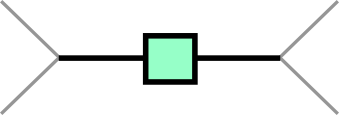
\includegraphics[scale = 0.4]{images/process}
  \caption{The \PD glyph for \glyph{process}.}
  \label{fig:process}
\end{figure}

A process is the basic process node in SBGN.  It describes a process that transforms a given set of biochemical entities---macromolecules, simple chemicals or unspecified entities---into another set of biochemical entities.  Such a transformation might imply modification of covalent bonds (conversion), modification of the relative position of constituents (conformational process) or movement from one compartment to another (translocation).

A cardinality label may be associated with \glyph{consumption} (\sect{consumption}) or \glyph{production} (\sect{production}) arcs to indicate the stoichiometry of the process.  This label becomes a requirement when the exact composition of the number of copies of the inputs or outputs to a reaction are ambiguous in the map.

A process is regarded as reversible if both `sides' of the process are connected to \glyph{production} arcs (see section \ref{sec: semantics reversible procs}).

The example in \fig{trans-phos} illustrates the use of a \glyph{process} node to represent the phosphorylation of a protein in a \PD.

\begin{figure}[H]
  \centering
  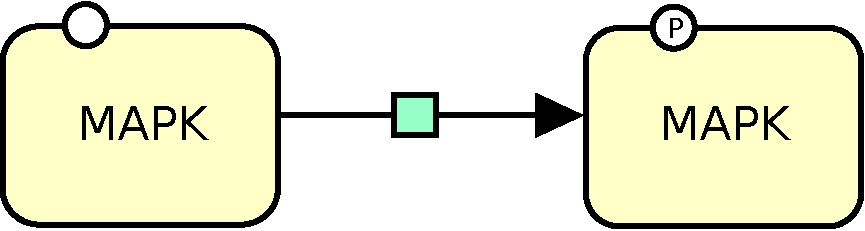
\includegraphics[scale = 0.3]{examples/process-phosphorylation}
  \caption{Phosphorylation of the protein MAP kinase.}
  \label{fig:trans-phos}
\end{figure}

The example in \fig{trans-react} illustrates the use of a \glyph{process} node to represent a reaction between two reactants that generates three products. 

\begin{figure}[H]
  \centering
  \includegraphics[scale = 0.3]{examples/process-reaction}
  \caption{Reaction between ATP and fructose-6-phosphate to produce fructose-1,6-biphosphate, ADP and a proton.}
  \label{fig:trans-react}
\end{figure}

The example in \fig{trans-trans} illustrates the use of a \glyph{process} node to represent a translocation. The large round-cornered rectangle represents a compartment border (see \sect{compartment}).

\begin{figure}[H]
  \centering
  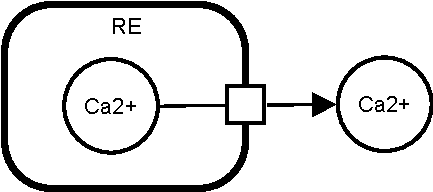
\includegraphics[scale = 0.3]{examples/process-translocation}
  \caption{Translocation of calcium ion out of the endoplasmic reticulum. Note that the \glyph{process} does not have to be located on the boundary of the \glyph{compartment}. A \glyph{process} is not attached to any \glyph{compartment}.}
  \label{fig:trans-trans}
\end{figure}

The example in \fig{trans-reverse} illustrates the use of a \glyph{process} node to represent the reversible opening and closing of an ionic channel in a \PD.

\begin{figure}[H]
  \centering
  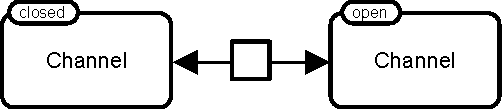
\includegraphics[scale = 0.3]{examples/process-reversible}
  \caption{Reversible opening and closing of an ionic channel.}
  \label{fig:trans-reverse}
\end{figure}

When such a reversible process is asymmetrically modulated, it must be represented by two different processes in a \PD.  \fig{trans-mod} illustrates the use of two \glyph{process} nodes to represent the reversible activation of a G-protein coupled receptor.  In the absence of any effector, an equilibrium exists between the inactive and active forms.  The agonist stabilises the active form, while the inverse agonist stabilises the inactive form.

\begin{figure}[H]
  \centering
  \includegraphics[scale = 0.3]{examples/process-modulated}
  \caption{The reversible activation of a G-protein coupled receptor.}
  \label{fig:trans-mod}
\end{figure}

The example in \fig{trans-dim} presents the conversion of two galactoses into a lactose.  Galactoses are represented by only one \glyph{simple chemical}, the cardinality being carried by the \glyph{consumption} arc.

\begin{figure}[H]
  \centering
  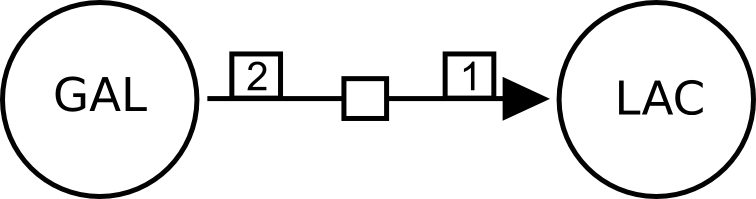
\includegraphics[scale = 0.3]{examples/process-dimerisation}
  \caption{Conversion of two galactoses into a lactose.}
  \label{fig:trans-dim}
\end{figure}




% The following is for [X]Emacs users.  Please leave in place.
% Local Variables:
% TeX-master: "../sbgn_PD-level1"
% End:

%%%%%%%%%%%%%%%%%%%%%%%%%%%%%%%%%%%%%%%%%%%%%%%%%%%%%%%%%%%%%%%%%%%%%%
%%                     Omitted Process
%%%%%%%%%%%%%%%%%%%%%%%%%%%%%%%%%%%%%%%%%%%%%%%%%%%%%%%%%%%%%%%%%%%%%%
%\color{blue}
\subsection{Glyph: \glyph{Omitted process}}\label{sec:omitted}

Omitted processes are processes that are known to exist, but are omitted from the map for the sake of clarity or parsimony. A single \glyph{omitted process} can represent any number of actual processes. For instance, one may want to represent a long chain of processes leading from one biochemical compound to another, without detailing all steps, but highlighting the fact that this is not a direct transformation.  The \glyph{omitted process} is different from a \glyph{submap} (\sect{submap}). While a \glyph{submap} references to an explicit content, that is hidden in the main map, the \glyph{omitted process} does not ``hide'' anything within the context of the map, and cannot be ``unfolded''. An \glyph{omitted process} is represented by a \glyph{process} in which the square box contains a two parallel slanted lines oriented northwest-to-southeast and separated by an empty space.

\begin{figure}[H]
  \centering
  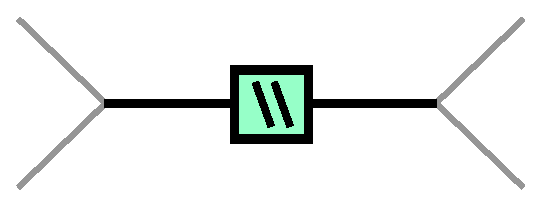
\includegraphics[scale = 0.5]{images/omitted}
  \caption{The \PD glyph for \glyph{omitted process}.}
  \label{fig:omitted}
\end{figure}




\subsection{Glyph: \glyph{Uncertain process}}
\label{sec:uncertain}

Uncertain processes are processes that may not exist. A single \glyph{uncertain process} can represent any number of actual processes.

\begin{glyphDescription}

\glyphSboTerm
SBO:0000396 ! uncertain process

\corr{\glyphOrigin
One or several \glyph{consumption} arcs (\sect{consumption}) or one or several \glyph{production} arcs (\sect{production}).
}{
\glyphIncoming
One or more \glyph{consumption} arcs (\sect{consumption})\footnote{Zero \glyph{consumption arcs} are allowed in the case of a reversible process.}, zero or more \glyph{modulation} arcs (\sect{modulations}).
}

\corr{\glyphTarget
One or several \glyph{production} arcs (\sect{production}).
}{
\glyphOutgoing
One or more \glyph{production} arcs (\sect{production}).
}

\glyphContainer
A \glyph{process} is represented by a square shape containing a question mark.
The shape is linked to two ports, that are small arcs attached to the centres of opposite sides of the shape, as shown in \fig{uncertain}.
The incoming \glyph{consumption} (\sect{consumption}) and outgoing \glyph{production} (\sect{production}) arcs are linked to the extremities of those ports.

The \glyph{modulation arcs} (\sect{modulations}) point to the other two sides of the shape.

\glyphLabel
\corr{An \glyph{uncertain process} is not identified by any label}{None}.

\glyphAux
\corr{An \glyph{uncertain process} does not carry any auxiliary items}{None}.

\end{glyphDescription}

\begin{figure}[H]
  \centering
  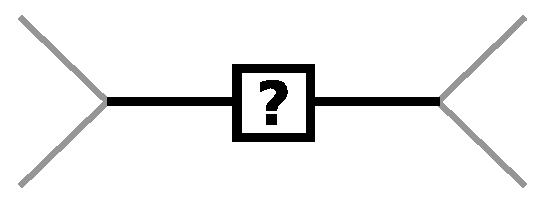
\includegraphics{images/uncertain}
  \caption{The \PD glyph for an \glyph{uncertain process}.}
  \label{fig:uncertain}
\end{figure}

\subsection{Glyph: \glyph{Association}}
\label{sec:association}

The \glyph{association} between one or more \glyph{EPNs} represents the non-covalent binding of the biological entities represented by those \glyph{EPNs} into a larger complex.

\begin{glyphDescription}

\glyphSboTerm
SBO:0000177 ! non-covalent binding

\corr{
\glyphOrigin One or more \glyph{consumption} arcs (\sect{consumption}).
}{
\glyphIncoming
One or more \glyph{consumption} arcs (\sect{consumption}), zero or more \glyph{modulation} arcs (\sect{modulations}).
}

\corr{
\glyphTarget  One \glyph{production} arc (\sect{production}).
One or several \glyph{production} arcs (\sect{production}).
}{
\glyphOutgoing
One \glyph{production} arc (\sect{production}).
}

\glyphContainer
An \glyph{association} is represented by a circular filled shape.
The shape is linked to two ports, that are small arcs attached to the centres of opposite sides of the shape, as shown in \fig{association}.
The incoming \glyph{consumption} (\sect{consumption}) and outgoing \glyph{production} (\sect{production}) arcs are linked to the extremities of those ports.

The \glyph{modulation arcs} (\sect{modulations}) point to the other two sides of the shape.

\glyphLabel
\corr{A \glyph{association} is not identified by any label}{None}.

\glyphAux
\corr{A \glyph{association} does not carry any auxiliary items}{None}.

\end{glyphDescription}

\begin{figure}[H]
  \centering
  \includegraphics{images/association}
  \caption{The \PD glyph for \glyph{association}.}
  \label{fig:association}
\end{figure}

The example in \fig{assoc-cyclin} illustrates the association of cyclin and CDC2 kinase into the Maturation Promoting Factor.

\begin{figure}[H]
  \centering
  \includegraphics[scale = 0.8]{examples/association-MPF}
  \caption{Association of cyclin and CDC2 kinase into the Maturation Promoting Factor.}
  \label{fig:assoc-cyclin}
\end{figure}

\fig{assoc-unamed} gives an example illustrating the association of a pentameric macromolecule (a nicotinic acetylcholine receptor) with a simple chemical (the local anesthetic chlorpromazin) in an unnamed complex.

\begin{figure}[H]
  \centering
  \includegraphics[scale = 0.8]{examples/association-unamed}
  \caption{The association of a pentameric macromolecule with a simple chemical in an unnamed complex.}
  \label{fig:assoc-unamed}
\end{figure}

An association does not necessarily result in the formation of a \glyph{complex}; it can also produce a \glyph{multimer}, or a \glyph{macromolecule} (although the latter case is semantically borderline).  \fig{assoc-multi} gives an example of this, using the formation of hemoglobin.

\begin{figure}[H]
  \centering
  \includegraphics[scale = 0.8]{examples/association-multimerisation}
  \caption{Formation of hemoglobin.}
  \label{fig:assoc-multi}
\end{figure}

% The following is for [X]Emacs users.  Please leave in place.
% Local Variables:
% TeX-master: "../sbgn_PD-level1"
% End:

%%%%%%%%%%%%%%%%%%%%%%%%%%%%%%%%%%%%%%%%%%%%%%%%%%%%%%%%%%%%%%%%%%%%%%
%%                     Dissociation
%%%%%%%%%%%%%%%%%%%%%%%%%%%%%%%%%%%%%%%%%%%%%%%%%%%%%%%%%%%%%%%%%%%%%%
%\color{blue}
\subsection{Glyph: \glyph{Dissociation}}\label{sec:dissociation}

The dissociation of an \glyph{EPN} into one or more \glyph{EPNs} represents the rupture of a non-covalent binding between the biological entities represented by those \glyph{EPNs}.

\begin{glyphDescription}
 \glyphSboTerm SBO:0000180 ! dissociation.
 \glyphOrigin One \glyph{consumption} arc (\sect{consumption}).
 \glyphTarget  One or more \glyph{production} arc (\sect{production}).
 \glyphNode A \glyph{dissociation} between several entities is represented by two concentric circles. A simple empty disc could be, in some cases, confused with the \glyph{catalysis} (section \sect{catalysis}). Moreover, the existence of two circles reminds the dissociation, by contrast with the filled disc of the \glyph{association} (\sect{association}).
 \end{glyphDescription}


\begin{figure}[H]
  \centering
  \includegraphics[scale = 0.5]{images/dissociation}
  \caption{The \PD glyph for \glyph{dissociation}.}
  \label{fig:dissociation}
\end{figure}

The example in \fig{dissoc-ribo} illustrates the dissociation of the small and large ribosomal subunits from a messenger RNA.

\begin{figure}[H]
  \centering
  \includegraphics[scale = 0.3]{examples/dissociation-ribosome}
  \caption{Dissociation of the small and large ribosomal subunits from a messenger RNA.}
  \label{fig:dissoc-ribo}
\end{figure}

\subsection{Glyph: \glyph{Phenotype}}
\label{sec:phenotype}

A biochemical network can generate phenotypes or affect biological processes.
Such processes can take place at different levels and are independent of the biochemical network itself.
To represent these processes in a map, \PD defines the \glyph{phenotype} glyph.

\begin{glyphDescription}

\glyphSboTerm
SBO:0000358 ! phenotype


\glyphIncoming
One or more \glyph{modulation} arcs (\sect{modulations}).



\glyphOutgoing
None.


\glyphContainer
A \glyph{phenotype} is represented by an elongated hexagonal shape, as shown in \fig{phenotype}.

\glyphLabel
A \glyph{phenotype} is identified by a label that is  a string of characters that may be distributed on several lines to improve readability.
The centre of the label must be placed on the centre of the shape.
The label may extend outside of the shape.

\glyphAux 
None.

\end{glyphDescription}

\begin{figure}[H]
  \centering
  \includegraphics{images/build/phenotype.pdf}
  \caption{The \PD glyph for \glyph{phenotype}.}
  \label{fig:phenotype}
\end{figure}

% The following is for [X]Emacs users.   Please leave in place.
% Local Variables:
% TeX-master: "../sbgn_PD-level1"
% End:


%%%%%%%%%%%%%%%%%%%%%%%%%%%%%%%%%%%%%%%%%%%%%%%%%%%%%%%%%%%%%%%%%%%%%%
%%%%%%%%%%%%%%%%%%%%%%%%%%%%%%%%%%%%%%%%%%%%%%%%%%%%%%%%%%%%%%%%%%%%%%
%%%%                  Arcs
%%%%%%%%%%%%%%%%%%%%%%%%%%%%%%%%%%%%%%%%%%%%%%%%%%%%%%%%%%%%%%%%%%%%%%
%%%%%%%%%%%%%%%%%%%%%%%%%%%%%%%%%%%%%%%%%%%%%%%%%%%%%%%%%%%%%%%%%%%%%%

% \section{Arcs}\label{sec:arcs}

% Arcs are lines that link \glyph{EPNs} and \glyph{PNs} together.  The symbols attached to their extremities indicate their semantics.


\section{Flux arcs}
\label{sec:fluxes}

Processes transform entity pools into other entity pools (\sect{PNs}).
Flux arcs allow representing which entity pools are consumed and produced by a process.
\glyph{Consumption} arcs link processes to their reactants, and \glyph{production} arcs link processes to their products.
\SBGNPDLone does not provide any specific arc to represent the fluxes of a reversible process, that can be conveniently represented using only \glyph{production} arcs.

\subsection{Glyph: \glyph{Consumption}}
\label{sec:consumption}

\glyph{Consumption} is the arc used to represent the fact that an entity pool is consumed by a process, but is not produced by the process.

\begin{glyphDescription}

\glyphSboTerm
SBO:0000394 ! consumption

\glyphOrigin
One \glyph{EPN} (\sect{EPNs}).

\glyphTarget
One \glyph{process node} (\sect{PNs}).

\glyphSymbol
No particular symbol is used to represent a \glyph{consumption}, as shown in \fig{consumption}.

\end{glyphDescription}

\begin{figure}[H]
  \centering
  \includegraphics{images/build/consumption.pdf}
  \caption{The \PD glyph for \glyph{consumption}.}
  \label{fig:consumption}
\end{figure}

A cardinality label may be associated with \glyph{consumption} (\sect{consumption}) or \glyph{production} (\sect{production}) arcs, indicating the stoichiometry of a process.
This label is a number enclosed in a rectangular container with one of the long sides adjacent to the \glyph{consumption} arc.
The cardinality is required to eliminate ambiguity when the exact composition, or the number of copies, of the inputs or outputs to a reaction are ambiguous from the map.
An example is a multimer of six subunits dissociating into two monomers and two dimers.
Without stoichiometry labels another result, such as four monomers and one dimer could be inferred.
Once assigned to one arc connecting to a process node, cardinality should be represented on all \glyph{consumption} and \glyph{production} arcs connected to that process node to avoid misinterpretation.

Omitted cardinality on one edge only should not be treated as cardinality of one, but as an unspecified cardinality.
In most cases, the exact value may be derived from the context, but unless cardinality is explicitly shown, it should be considered as unspecified.
In the case where the stoichiometry of some part of the process is not known, or undefined, a question mark ("?") should be used within the cardinality label of the corresponding arcs.

\subsection{Glyph: \glyph{Production}}
\label{sec:production}

\glyph{Production} is the arc used to represent the fact that an entity pool is produced by a process. In the case of a reversible process, the \glyph{production} arc \corr{also acts as a \glyph{consumption} arc}{represents both a consumption and a production}.

\begin{glyphDescription}

\glyphSboTerm
SBO:0000393 ! production

\glyphOrigin
\corr{Any}{One} \glyph{process node} (\sect{PNs}).

\glyphTarget
\corr{Any}{One} \glyph{EPN} (\sect{EPNs}).

\glyphSymbol
The target extremity of a \glyph{production} carries a filled arrowhead, as shown in \fig{production}.

\end{glyphDescription}

\begin{figure}[H]
  \centering
  \includegraphics{images/production}
  \caption{The \PD glyph for \glyph{production}.}
  \label{fig:production}
\end{figure}

A cardinality label may be associated with a \glyph{production} arc, indicating the stoichiometry of a process.

\fig{prod-card} illustrates the use of \corr{consumption/production}{\glyph{consumption}/\glyph{production}} arc cardinality labels to represent the stoichiometry of a process.

\begin{figure}[H]
  \centering
  \includegraphics[scale = 0.6]{examples/stoichEx1}
  \caption{Cardinality for production arcs.
  \add{The process on the top is wrong as the stoichiometry is not represented, which leads to ambiguity.}}
  \label{fig:prod-card}
\end{figure}

% The following is for [X]Emacs users.  Please leave in place.
% Local Variables:
% TeX-master: "../sbgn_PD-level1"
% End:


\section{Modulation arcs}
\label{sec:modulations}

Modulation arcs represent influences of entity pools on processes.
A stimulation affects positively the flux of a process, while an inhibition affects it negatively.
\SBGNPDLone provides six modulation arcs: \glyph{modulation}, \glyph{stimulation}, \glyph{catalysis}, \glyph{necessary stimulation} and \glyph{inhibition}.

\subsection{Glyph: \glyph{Modulation}}
\label{sec:modulation}

% A modulation affects the flux of a process
% represented by the target process. Such a modulation can affect the
% process \textbf{positively or negatively}, or even both ways depending on the
% conditions, for instance the concentration of the intervening
% participants. A \glyph{modulation} can also be used when one does not know the precise direction of the effect.

A general modulation where the exact nature of the modulation is not specified or not known.
The \glyph{modulation} glyph can be used when one does not know the precise direction of the effect.

\begin{glyphDescription}

\glyphSboTerm
SBO:0000168 ! control

\glyphOrigin
One \glyph{EPN} (\sect{EPNs}) or  \glyph{logical operator} (\sect{logic}).

\glyphTarget
One \glyph{process node} (\sect{PNs}).

\glyphSymbol
The target extremity of a \glyph{modulation} carries an empty diamond, as shown in \fig{modulation}.

\end{glyphDescription}

\begin{figure}[H]
  \centering
  \includegraphics{images/build/modulation.pdf}
  \caption{The \PD glyph for \glyph{modulation}.}
  \label{fig:modulation}
\end{figure}

\fig{modul-nico} represents the effect of nicotine on the process between closed and open states of a nicotinic acetylcholine receptor. High concentrations of nicotine open the receptor while low concentrations can desensitize it without opening.

\begin{figure}[H]
  \centering
  \includegraphics[scale = 0.8]{images/build/modulation_nAChR_example.pdf}
  \caption{Modulation of nicotinic receptor opening by nicotine.}
  \label{fig:modul-nico}
\end{figure}

\subsection{Glyph: \glyph{Stimulation}}
\label{sec:stimulation}

A stimulation affects \textbf{positively} the flux of a process represented by the target process.
This stimulation can be, for instance, a catalysis or a positive allosteric regulation. Note that \glyph{catalysis} exists independently in SBGN, see \sect{catalysis}.

\begin{glyphDescription}

\glyphSboTerm
SBO:0000170 ! stimulation

\glyphOrigin
One \glyph{EPN} (\sect{EPNs}) or  \glyph{logical operator} (\sect{logic}).

\glyphTarget
One \glyph{process node} (\sect{PNs}).

\glyphSymbol
The target extremity of a \glyph{stimulation} carries an empty arrowhead, as shown in \fig{stimulation}.

\end{glyphDescription}

\begin{figure}[H]
  \centering
  \includegraphics{images/build/stimulation.pdf}
  \caption{The \PD glyph for \glyph{stimulation}.}
  \label{fig:stimulation}
\end{figure}

%%%%%%%%%%%%%%%%%%%%%%%%%%%%%%%%%%%%%%%%%%%%%%%%%%%%%%%%%%%%%%%%%%%%%%
%%                     Catalysis
%%%%%%%%%%%%%%%%%%%%%%%%%%%%%%%%%%%%%%%%%%%%%%%%%%%%%%%%%%%%%%%%%%%%%%
%\color{blue}
\subsection{Glyph: \glyph{Catalysis}}\label{sec:catalysis}

A catalysis is a particular case of stimulation, where the effector affects
positively the flux of a process represented by the target process. The positive effect on the process is due to the lowering of the activation energy of a reaction. The target extremity of a \glyph{catalysis} carries an empty circle.

\begin{figure}[H]
  \centering
  \includegraphics[scale = 0.5]{images/catalysis}
  \caption{The \PD glyph for \glyph{catalysis}.}
  \label{fig:catalysis}
\end{figure}

The example in \fig{catalysis-MAPK} illustrates the use of \glyph{catalysis} arc to represent the effect of MAPKK on the phophorylation of MAPK.

\begin{figure}[H]
  \centering
  \includegraphics[scale = 0.5]{images/catalysis-MAPK}
  \caption{MAPKK catalyses the phosphorylation of MAPK.}
  \label{fig:catalysis-MAPK}
\end{figure}

\subsection{Glyph: \glyph{Inhibition}}
\label{sec:inhibition}

An inhibition \textbf{negatively} affects the flux of a process represented by the target process.
This inhibition can be, for instance, a competitive inhibition or an allosteric inhibition.

\begin{glyphDescription}

\glyphSboTerm
SBO:0000169 ! inhibition

\glyphOrigin
One \glyph{EPN} (\sect{EPNs}) or \glyph{logical operator} (\sect{logic}).

\glyphTarget
One \glyph{process node} (\sect{PNs}).

\glyphSymbol
The target extremity of an \glyph{inhibition} carries a bar perpendicular to the arc, as shown in \fig{inhibition}.

\end{glyphDescription}

\begin{figure}[H]
  \centering
  \includegraphics{images/build/inhibition.pdf}
  \caption{The \PD glyph for \glyph{inhibition}.}
  \label{fig:inhibition}
\end{figure} 

\subsection{Glyph: \glyph{Necessary stimulation}}
\label{sec:necessary_stim}

A necessary stimulation is one that is necessary for a process to take place. A process modulated by a necessary stimulation can only occur when this necessary stimulation is active.

\begin{glyphDescription}

\glyphSboTerm
SBO:0000171 ! necessary stimulation

\glyphOrigin
One \glyph{EPN} (\sect{EPNs}) or \glyph{logical operator} (\sect{logic}).

\glyphTarget
One \glyph{process node} (\sect{PNs}).

\glyphSymbol
The target extremity of a \glyph{necessary stimulation} carries an open arrowhead (to remind that it is a \glyph{stimulation}) coming after a larger perpendicular bar, as shown in \fig{Necessary Stimulation}.

\end{glyphDescription}

\begin{figure}[H]
  \centering
  \includegraphics{images/build/necessary_stim.pdf}
  \caption{The \PD glyph for \glyph{Necessary Stimulation}.}
  \label{fig:Necessary Stimulation}
\end{figure}

The example in \fig{necessary_stim-gene} below describes the transcription of a gene~X, that is the creation of a messenger RNA~X triggered by the gene~X.  The creation of the protein~X is then triggered by the mRNA~X.  (Note that the same example could be represented using the gene as reactant and product, although it is semantically different.)

\begin{figure}[H]
  \centering
  \includegraphics[scale = 0.8]{images/build/necessary_stim_genetic_example.pdf}
  \caption{The creation of a messenger RNA~X triggered by the gene~X.}
  \label{fig:necessary_stim-gene}
\end{figure}

The example in \fig{necessary_stim-calcium} below describes the transport of calcium ions out of the endoplasmic reticulum. Without IP3 receptor, there is no calcium flux, therefore, one cannot use a \glyph{stimulation}.
The \glyph{necessary stimulation} instead represents the necessity for the receptor to be present for the transport to take place.

\begin{figure}[H]
  \centering
  \includegraphics[scale = 0.8]{images/build/necessary_stim_transport_example.pdf}
  \caption{The transport of calcium ions out of the endoplasmic reticulum into the cytosol. Note that IP3R crosses both compartment boundaries. This is allowed, but the Macromolecule should only belong to one of the compartments see section \ref{sec: unresolved multi-comp ents} for more discussion of this issue.}
  \label{fig:necessary_stim-calcium}
\end{figure}


%%%%%%%%%%%%%%%%%%%%%%%%%%%%%%%%%%%%%%%%%%%%%%%%%%%%%%%%%%%%%%%%%%%%%%
%%%%%%%%%%%%%%%%%%%%%%%%%%%%%%%%%%%%%%%%%%%%%%%%%%%%%%%%%%%%%%%%%%%%%%
%%%%                   Logical operators
%%%%%%%%%%%%%%%%%%%%%%%%%%%%%%%%%%%%%%%%%%%%%%%%%%%%%%%%%%%%%%%%%%%%%%
%%%%%%%%%%%%%%%%%%%%%%%%%%%%%%%%%%%%%%%%%%%%%%%%%%%%%%%%%%%%%%%%%%%%%%

\section{Logical operators}

\label{sec:logic}

The \glyph{logical operator} performs an operation on one or more inputs to give a unique output.
The \glyph{and}, \glyph{or}, and \glyph{not} operators perform a Boolean operation to give a binary output, while the \glyph{equivalence} operator performs a union of pools to give a new pool.


\subsection{Glyph: \glyph{And}}
\label{sec:and}


The output of an \glyph{and} glyph is True if all its inputs are True, and False otherwise.



\begin{glyphDescription}

\glyphSboTerm
SBO:0000173 ! and


\glyphIncoming One or more \glyph{logic arcs} (\sect{logicArc}).



\glyphOutgoing
One \glyph{logic arc} (\sect{logicArc}) or \glyph{modulation arc} (\sect{modulations}).


\glyphContainer
An \glyph{and} operator is represented by a circular shape containing the word ``AND''.
The shape is linked to two ports, that are small arcs attached to the centres of opposite sides of the shape, as shown in \fig{and}.
The incoming \glyph{logic arcs} (\sect{logicArc}) are linked to the extremity of the leftmost or uppermost port, while the outgoing \glyph{logic arc} (\sect{logicArc}) or \glyph{modulation} (\sect{modulation}) is linked to the extremity of the rightmost or bottommost port.

\glyphLabel
None.

\glyphAux
None.

\end{glyphDescription}

\begin{figure}[H]
  \centering
  \includegraphics{images/build/and.pdf}
  \caption{The \PD glyph for \glyph{and}. Only two inputs are represented, but more would be allowed.}
  \label{fig:and}
\end{figure}

% The following maps illustrate the dephosphorylation of the MAP inase ERK by the protein phosphatase 2A and the STriatal Enriched Phosphatase, in ST (left) and ER (right).
%
% \begin{center}
% \scalebox{0.5}{\includegraphics{images/build/stimulation_example1}.pdf}
% \end{center}

\subsection{Glyph: \glyph{Or}}
\label{sec:or}

\corr{The glyph \glyph{or} is used to denote that any of the \glyph{EPNs} linked as input is sufficient to produce the output.}
{
The output of an \glyph{or} glyph is True if at least one of its inputs is True, and False otherwise.
}

\begin{glyphDescription}

\glyphSboTerm
SBO:0000174 ! or

\corr{
\glyphOrigin More than one \glyph{EPN} (section~\ref{sec:EPNs}) or \glyph{logical operator} (section~\ref{sec:logic}).
}{
\glyphIncoming One or more \glyph{logic arcs} (\sect{logicArc}).
}

\corr{
\glyphTarget  One modulation (section~\ref{sec:modulation}), stimulation (section~\ref{sec:stimulation}), catalysis (section~\ref{sec:catalysis}), inhibition (section~\ref{sec:inhibition}) or necessary stimulation (section~\ref{sec:necessary_stim}) arc.
}{
\glyphOutgoing
One \glyph{logic arc} (\sect{logicArc}) or \glyph{modulation arc} (\sect{modulations}).
}

\glyphContainer
An \glyph{or} operator is represented by a circular shape containing the word ``OR''.
The shape is linked to two ports, that are small arcs attached to the centres of opposite sides of the shape, as shown in \fig{or}.
The incoming \glyph{logic arcs} (\sect{logicArc}) are linked to the extremity of the leftmost or uppermost port, while the outgoing \glyph{logic arc} (\sect{logicArc}) or \glyph{modulation} (\sect{modulation}) is linked to the extremity of the rightmost or bottommost port.

\glyphLabel
\corr{An \glyph{or} operator is not identified by any label}{None}.

\glyphAux
\corr{An \glyph{or} operator does not carry any auxiliary items}{None}.

\end{glyphDescription}

\begin{figure}[H]
  \centering
  \includegraphics{images/or}
  \caption{The \PD glyph for \glyph{or}. Only two inputs are represented, but more would be allowed.}
  \label{fig:or}
\end{figure}

%%%%%%%%%%%%%%%%%%%%%%%%%%%%%%%%%%%%%%%%%%%%%%%%%%%%%%%%%%%%%%%%%%%%%%
%%                     Not
%%%%%%%%%%%%%%%%%%%%%%%%%%%%%%%%%%%%%%%%%%%%%%%%%%%%%%%%%%%%%%%%%%%%%%
%\color{blue}
\subsection{Glyph: \glyph{Not}}\label{sec:not}

The glyph \glyph{not} is used to denote that the \glyph{EPN} linked as input cannot produce the output. \glyph{Not} is represented by a circle carrying the word ``NOT''.

\begin{figure}[H]
  \centering
  \includegraphics[scale = 0.5]{images/not}
  \caption{The \PD glyph for \glyph{not}.}
  \label{fig:not}
\end{figure}


\subsection{Glyph: \glyph{Equivalence}}
\label{sec:equivalence}
%The glyph \glyph{equivalence} is used to denote that all the \glyph{EPNs} linked as input are necessary to produce the output.  
\add{The \glyph{equivalence operator} provides a mechanism to sub-class EPNs. For example, this operator allows specifying that macromolecules or nucleic acid features X\textsubscript{1}, X\textsubscript{2}, and X\textsubscript{3} are subclasses of X. This avoids the need for processes that apply to all subtypes of X to be duplicated and simplifies cases where combinatorial explosions of the number of EPNs or PNs may arise. Caution should be used with this glyph as there is the possibility that ambiguity may be introduced into a SBGN map. Examples of the correct usage of this glyph are provided in Appendix~\ref{ex_eq} together with examples of misuse along with a proposed set of guidelines for the use of this \glyph{equivalence operator}.}

\luna{this section is written very differently from the others. text like "until now" may have no purpose years later when people read this. TEXT BEFORE 032819: 
Until now, the SBGN Process Description language has not provided mechanisms to sub-class EPNs.
There was no specific means of specifying that macromolecules or nucleic acid features \corr{X1}{X\textsubscript{1}}, \corr{X2}{X\textsubscript{2}}, and \corr{X3}{X\textsubscript{3}} are subclasses of X.
Therefore, any process that applies to all the subtypes of X had to be triplicated.
That situation could easily generate combinatorial explosions of the number of EPNs or PNs.

To enable the representation of EPNs together with corresponding sub-classes of this EPNs, we introduce the equivalence operator glyph.
Please note that this glyph can potentially introduce ambiguity.
Examples of the correct use of the glyph are provided in Appendix~\ref{ex_eq} together with examples of misuse and with the proposed set of rules suggested as guideline for the use of the \glyph{equivalence operator}.}

\begin{glyphDescription}

\glyphSboTerm
SBO:0000392 ! equivalence\corr{ (is a)}{}

\corr{
\glyphOrigin More than one \glyph{EPN} (section~\ref{sec:EPNs}).
}{
\glyphIncoming Two or more \glyph{logic arcs} (\sect{logicArc}).
}

\corr{
\glyphTarget  One logic arc (section~\ref{sec:logicArc}).
}{
\glyphOutgoing
One \glyph{logic arc} (\sect{logicArc}).
}

\glyphContainer
An \glyph{equivalence} operator is represented by a circular shape containing the symbol ``$\Xi$'' (letter ``xi'' of the Greek alphabet\add{)}.
The choice of the symbol is motivated by its use in mathematics for describing relationships as ``equivalent to'' or ``identical to''.
% \rougny{In my opinion, this shows that the equivalence operator should not be a logical operator (and even not an operator at all), because it represents a relationship (it does not produce anything, on the contrary to operators)}
The shape is linked to two ports, that are small arcs attached to the centres of opposite sides of the shape, as shown in \fig{equivalenceOperator}.
\corr{The incoming \glyph{logic arcs} (\sect{logicArc}) are linked to the extremity of the leftmost or uppermost port, while the outgoing \glyph{logic arc} (\sect{logicArc}) is linked to the extremity of the rightmost or bottommost port.}{}

\glyphLabel
\corr{An \glyph{equivalence} operator is not identified by any label}{None}.

\glyphAux
\corr{An \glyph{equivalence} operator does not carry any auxiliary items}{None}.

\end{glyphDescription}

\begin{figure}[H]
  \centering
  \includegraphics{images/equivalence}
  \caption{The \PD glyph for \glyph{equivalence operator}. Only two inputs are represented, but more would be allowed.}
  \label{fig:equivalenceOperator}
\end{figure}

\add{
The example of \fig{D1_1} presents the binding of different forms of TNF$\alpha$ to two receptors, TNFR1 and TNFR2.
Only membrane TNF$\alpha$ (mTNF$\alpha$) can bind to TNFR2, while both membrane TNF$\alpha$ and soluble TNF$\alpha$ (sTNF$\alpha$) can bind to TNFR1.
Binding of both forms to TNFR1 can conveniently be represented using a generic form of TNF$\alpha$, that is built using an \glyph{equivalence operator}.
}

\begin{figure}
\begin{center}
\includegraphics[scale=0.45]{examples/D1_1}
\end{center}
\caption{Binding of diverse forms of TNF$\alpha$ to TNF receptors.}
\label{fig:D1_1}
\end{figure}



% \begin{center}
% \scalebox{0.5}{\includegraphics{images/stimulation-example1}}
% \end{center}


\section{Logic arc}
\label{sec:logic_arc}

\subsection{Glyph: \glyph{Logic arc}}
\label{sec:logicArc}

\glyph{Logic arc} is used to represent the fact that an entity pool or a logical operator influences
the outcome of a logic operator.

\begin{glyphDescription}

\glyphSboTerm
SBO:0000398 ! logical relationship

\glyphOrigin
One \glyph{EPN} (\sect{EPNs}) or \glyph{logical operator} (\sect{logic}).

\glyphTarget
One \glyph{logical operator} (\sect{logic}) or \glyph{EPN} (\sect{EPNs}).

\glyphSymbol
No particular symbol is used to represent a \glyph{logic arc}, as shown in \fig{logicArc}.

\end{glyphDescription}

\begin{figure}[H]
  \centering
  \includegraphics{images/build/logic_arc.pdf}
  \caption{The \PD glyph for \glyph{logic arc}.}
  \label{fig:logicArc}
\end{figure}


\section{Annotating nodes and arcs}

\subsection{Glyph: \glyph{Annotation}}
\label{sec:annotation}

In \SBGNPDLone there are cases where the language does not capture everything the author wishes to convey.
This may be additional experimental detail or descriptions of mechanisms that cannot be fully described by the \PDl.
In this case the language provides the \glyph{annotation} glyph. This contains text and is associated with a particular glyph in a map.
Importantly, it is purely ``decoration'' and does alter the meaning the map.

\begin{glyphDescription}

\glyphSboTerm
SBO:0000550 ! annotation


\glyphIncoming
None.



\glyphOutgoing
None.


\glyphContainer
An \glyph{annotation} is represented by a rectangular shape with a folded corner, as shown in \fig{techref:annotation}.
This shape is linked to the annotated element via a callout (see Figure \ref{fig:techref:ex-annotation}).
The callout should overlap with the object it is annotating.

\glyphLabel
An \glyph{annotation} is identified by a label that is  a string of characters that may be distributed on several lines to improve readability.
The centre of the label must be placed on the centre of the shape.

\glyphAux
None.

\end{glyphDescription}

\begin{figure}[htb]
  \centering
  \includegraphics{images/annotation}
  \caption{The \PD glyph for \glyph{annotation}.}
  \label{fig:techref:annotation}
\end{figure}

\begin{figure}[htb]
  \centering
  \includegraphics[scale = 0.8]{examples/ex-annotation}
  \caption{Example of \glyph{annotations} adding information to the
    description of the trans-phosphorylation of CaMKII. Note that
    three different types of links are used between annotation nodes
    and annotated elements. However, it is recommended to use a
    consistent scheme within a map.}
  \label{fig:techref:ex-annotation}
\end{figure}


\section{Referring to other nodes}
\label{sec:ref_nodes}

Reference nodes handle links or relationships between elements of a map and sub-map.
At present there is only one reference glyph, \glyph{tag}, which can be used in a map referred to by a \glyph{submap} (\sect{submap}).


% $HeadURL$

\subsection{Glyph: \glyph{Tag}}
\label{sec:tag}

A \glyph{tag} is a named handle, or reference, to another EPN (\sect{EPNs}) or compartment (\sect{compartment}).  \glyph{Tags} are used to identify those elements in \glyph{submaps} (\sect{submap}).

\begin{glyphDescription}

\glyphSboTerm Not applicable.

\glyphContainer A \glyph{tag} is represented by a rectangle fused to an empty arrowhead, as illustrated in \fig{tag}.  The symbol should be linked to one and only one edge (\ie it should reference only one EPN or compartment).

\glyphLabel A \glyph{tag} is identified by a label placed in an unbordered box containing a string of characters.  The characters can be distributed on several lines to improve readability, although this is not mandatory.  The label box must be attached to the center of the container. The label may spill outside of the container.

\glyphAux A \glyph{tag} does not carry any auxiliary items. 

\end{glyphDescription}

\begin{figure}[H]
  \centering
  \includegraphics[scale = 0.3]{images/tag}
  \caption{The \PD glyph for \glyph{tag}.}
  \label{fig:tag}
\end{figure}




% The following is for [X]Emacs users.   Please leave in place.
% Local Variables:
% TeX-master: "../sbgn_PD-level1"
% End:


\subsection{Glyph: \glyph{Equivalence arc} }\label{sec:equivalenceArc}

An \glyph{equivalence arc} is used to link a \glyph{tag} (\sect{tag}) or a \glyph{submap terminal} (\sect{submapTerminal}) to the \glyph{EPN} (\sect{EPNs}) or \glyph{compartment} (\sect{compartment}) it refers to.

\begin{glyphDescription}

\glyphSboTerm
Not applicable.

\glyphOrigin
One \glyph{EPN} (\sect{EPNs}) or \glyph{compartment} (\sect{compartment}).

\glyphTarget
One \glyph{tag} (\sect{tag}) or \glyph{submap terminal} (\sect{submapTerminal}).

\glyphSymbol No particular symbol is used to represent an \glyph{equivalence arc}, as shown in \fig{equivalenceArc}.
 \end{glyphDescription}

\begin{figure}[H]
  \centering
  \includegraphics[scale = 0.8]{images/build/equivalence_arc.pdf}
  \caption{The \PD glyph for \glyph{Equivalence arc}.}
  \label{fig:equivalenceArc}
\end{figure}


%%%%%%%%%%%%%%%%%%%%%%%%%%%%%%%%%%%%%%%%%%%%%%%%%%%%%%%%%%%%%%%%%%%%%%
%%%%%%%%%%%%%%%%%%%%%%%%%%%%%%%%%%%%%%%%%%%%%%%%%%%%%%%%%%%%%%%%%%%%%%
%%%%                   Submap
%%%%%%%%%%%%%%%%%%%%%%%%%%%%%%%%%%%%%%%%%%%%%%%%%%%%%%%%%%%%%%%%%%%%%%
%%%%%%%%%%%%%%%%%%%%%%%%%%%%%%%%%%%%%%%%%%%%%%%%%%%%%%%%%%%%%%%%%%%%%%

\section{Encapsulation}
\label{sec:encapsulation}
\subsection{\glyph{Submap}}\label{sec:submap}

A \glyph{submap} is used to encapsulate a map (including all types of nodes and edges) within one glyph.
As such, it is not equivalent to an \glyph{omitted process} (\sect{omitted}).
The \glyph{submap} hides the content of this map to the users, and displays only \glyph{submap terminals} (\sect{submapTerminal}).
In the case of an SBGN description that is made available through a software tool, the map enclosed by the  \glyph{submap} may be available to the tool.
A user could then ask the tool to expand this map in a different canvas, for instance by clicking on the \glyph{submap}.
In the case of an SBGN description made available in a book or a website, the content of the map may be available on another page, possibly accessible via an hyperlink on the \glyph{submap}.

\begin{glyphDescription}

\glyphSboTerm
SBO:0000395 ! encapsulating process

\glyphIncoming
None.

\glyphOutgoing
None.

\glyphContainer
A \glyph{submap} is represented by a rectangular shape, to remind that it is fundamentally a process.

\glyphLabel
A \glyph{submap} is identified by a label that is an unbordered box containing a string of characters.
The characters may be distributed on several lines to improve readability.
The centre of the label must be placed on the centre of the shape.
The label may extend outside of the shape.

\glyphAux
A \glyph{submap} must carry one or more \glyph{submap terminals} (\sect{submapTerminal}), each linked to an \glyph{EPN} (\sect{EPNs}) or \glyph{compartment} (\sect{compartment}) of the map using an \glyph{equivalence arc} (\sect{equivalenceArc}).

\end{glyphDescription}

\begin{figure}
\begin{center}
\includegraphics[scale=0.7]{images/build/submap.pdf}
\caption{The \PD glyph for \glyph{submap}, shown plain and unadorned on the left, and with three \glyph{submap terminals} on the right.}
\label{fig:submap}
\end{center}
\end{figure}

\fig{folded} represents a \glyph{submap} that encapsulates processes transforming glucose into fructose-6-phosphate.
The \glyph{submap} carries five \glyph{submap terminals}, four linked to \glyph{EPNs} and one linked to a \glyph{compartment}.
The latter is particularly important in the case of \glyph{EPNs} present only in a \glyph{compartment} enclosed in a \glyph{submap}, and that are not linked to \glyph{submap terminals} themselves.
Note that the \glyph{submap terminals} do not allow defining a ``direction'' for the flux of the processes enclosed in the \glyph{submap}, which is solely determined by the context as in \fig{folded}.

\begin{figure}
\begin{center}
\includegraphics[scale=0.8]{images/build/submap_folded_example.pdf}
\caption{Example of a \glyph{submap} encapsulating processes that transform glucose into fructose-6-phosphate.
The map enclosed by the \glyph{submap} is shown in \fig{unfolded}, whose \glyph{tags} are referred to by the \glyph{submap terminals} decorating the present \glyph{submap} glyph.
}
\label{fig:folded}
\end{center}
\end{figure}

The map in \fig{unfolded} represents the map enclosed in the \glyph{submap} of \fig{folded}.
Note that the tag 5 links the mitochondria \glyph{compartment} in this map to the mitochondria \glyph{compartment} of the main map in \fig{unfolded}.

The \glyph{compartment} containing glucose-6-phosphate is implicitly defined as the same as the \glyph{compartment} containing glucose and fructose-6-phosphate.
There is no ambiguity because if glucose and fructose-6-phosphate were in different \glyph{compartments}, at least one of them would have been linked to a \glyph{submap terminal} of the \glyph{submap} of \fig{folded}.

\begin{figure}
\begin{center}
\includegraphics[scale=0.8]{images/build/submap_unfolded_example.pdf}
\caption{Example of a map with \glyph{tags}, showing that it is enclosed in a \glyph{submap} of another map (here, the one of \fig{folded}).}
\label{fig:unfolded}
\end{center}
\end{figure}


% The following is for [X]Emacs users.  Please leave in place.
% Local Variables:
% TeX-master: "../sbgn_PD-level1"
% End:
